%% --------------------------------------------------------------------
%% thesis.tex -- MAIN FILE (the one that you compile with LaTeX)
%% --------------------------------------------------------------------
%% version 1.8.09.02.16 (beta)

%-----<<<<<<<<<<<< START >>>>>>>>>>>>-----
\documentclass [a4paper,12pt]{report}  
\usepackage[a-2u]{pdfx}      		
\usepackage[cp1250]{inputenc}																	%cp1250 for Czechoslovak characters, utf8
\usepackage{lmodern}
\usepackage[T1]{fontenc}
\usepackage{textcomp}

%-----<<< --------------------------------- >>>-----

%-----<<<<<<<<<<<< DEFINITIONS >>>>>>>>>>>>----- % for special characters of Czech/Slovak lang. use LaTeX commands only such as accute accent \'{o}, caron over the letter \v{s}, etc..
\def \BookName {Bachelor's thesis}
\def \Bookname {Noise reduction and feature extraction with principal component analysis for cryptocurrency price modeling}
\def \BooknameCZ {Redukce \v{s}umu a extrakce rys\r{u} pomoc\'{i} anal\'{y}zy hlavn\'{i}ch komponent pro modelov\'{a}n\'{i} cen kryptom\v{e}n} 
\def \AutorDP {Tom\'{a}\v{s} Barho\v{n}}													
\def \AuthorDP {Tomas Barhon} 			%here use just English characters!
\def \FirstNameDP {Tom\'{a}\v{s}} 				
\def \LastNameDP {Barho\v{n}} 							
\def \Email {tomas.barhon@hotmail.cz}
\def \Year {2024}
\def \Place {Prague}
\def \Subject {Price Elasticity of Gasoline Demand}
\def \Keywords {Cryptocurrency, Bitcoin, Ethereum, Litecoin, Machine Learning, PCA, Noise Reduction}
\def \Klic {Kryptoměny, Bitcoin, Ethereum, Litecoin, Strojové učení, PCA, Redukce šumu} 					
\def \JEL {\href{http://ideas.repec.org/j/C01.html}{C01},			%http://www.aeaweb.org/journal/elclasjn_hold.html
 \href{https://ideas.repec.org/j/G00.html}{G00},								%change the codes in the argument and also in the URL
 \href{http://ideas.repec.org/j/F23.html}{F23},
 \href{http://ideas.repec.org/j/H25.html}{H25}, 	
 \href{http://ideas.repec.org/j/H71.html}{H71},
 \href{http://ideas.repec.org/j/H87.html}{H87}}	
\def \Thesisweb {\href{https://github.com/Tomas-Barhon/Noise-reduction-and-feature-extraction-with-principal-component-analysis}}		%thesis webpage (leave empty if you use none)
\def \AcademicYear {2023/2024}
\def \Supervisor {prof. PhDr. Ladislav Kri\v{s}toufek Ph.D.}
\def \StudyProgram {Economics and Finance}
\def \EmailSup {ladislav.kristoufek@fsv.cuni.cz}
\def \CUNI {Charles University}
\def \FSS {Faculty of Social Sciences}
\def \IES {Institute of Economic Studies}
%-----<<< --------------------------------- >>>-----

%-----<<< METADATA >>>-----%filecontents must be in form of text, do not put definition reference like ``\AuthorDP'' inside
%\usepackage{filecontents}
%\begin{filecontents*}{Thesis.xmpdata}
%		\Author{Firstname Lastname} 
%		\Title{The Price Elasticity of Gasoline Demand: A Meta-Analysis}
%		\Keywords{keywordone, keywordtwo, keywordthree, keywordfour}
%		\Subject{Price Elasticity of Gasoline Demand}
%		\Publisher{Charles University} 
%\end{filecontents*} 

%-----<<<<<<<<<<<< STYLES >>>>>>>>>>>>-----      														
\usepackage{Styles/Head}
\usepackage{Styles/Mystyle}	
%-----<<< --------------------------------- >>>-----

%-----<<<<<<<<<<<< DOCUMENT >>>>>>>>>>>>-----
\begin{document}
\frontmatter                   									%lowercase roman pagination for front matter
\clubpenalty 9999 															%not so many orphants
\widowpenalty 9999 															%not so many widows

%-----<<< HEAD >>>-----
\pagestyle{empty}                       				%no visible pagination here                    
\BookHead
%-----<<< ---- >>>-----

%-----<<< DECLARATION >>>-----
\vfill

\vglue 14cm

\section*{Declaration of Authorship}
The author hereby declares that he compiled this thesis independently, using only the listed resources and literature, and the thesis has not been used to obtain any other academic title.

\bigskip 

\noindent The author grants to Charles University permission to reproduce and to distribute copies of this thesis in whole or in part and agrees with the thesis being used for study and scientific purposes.
\vspace{0.5cm}

\begin{table}[!hbp]
\begin{tabular}{lr}
\hspace{-0.3cm} Prague, \today
\hspace{3cm}       
 \begin{tabular}{p{4.5cm}}
    \vspace{0.6cm} \\
     \hline \\ 
		\vspace{-0.7cm} \hspace{0.6cm} \AuthorDP
 \end{tabular}

\end{tabular}
\end{table}
        					%input file
\clearpage
%-----<<< ----------- >>>-----


%-----<<< ABSTRACT >>>-----
\phantomsection													 				%bookmark anchor
\pdfbookmark[0]{Abstract}{abst}        	 				%add bookmark
\section*{Abstract}

The abstract should concisely summarize the
contents of a thesis. Since potential readers should be able to
make their decision on the personal relevance based on the abstract,
the abstract should clearly tell the reader what information
he can expect to find in the thesis. The most essential issue
is the problem statement and the actual contribution of described
work. The authors should always keep in mind that the
abstract is the most frequently read part of a thesis. It should
contain at least 70 and at most 120 words (200 when you are writing a thesis).
Do not cite anyone in the abstract.

\bigskip

\begin{tabular}{lp{8.6cm}}
		\textbf{JEL Classification} & \JEL \\
		\textbf{Keywords} & \Keywords \\
 		& \\
		\textbf{Title} & \Bookname \\
 		\textbf{Author's e-mail} & \texttt{\href{mailto:\Email}{\Email}}\\
		\textbf{Supervisor's e-mail} & \texttt{\href{mailto:\EmailSup}{\EmailSup}}\\
\end{tabular}

\bigskip

\section*{Abstrakt}\label{abstract}

Nutnou sou��st� pr�ce je anotace, kter� shrnuje v�znam pr�ce a v�sledky v n� dosa�en�. Anotace pr�ce by nem�la b�t del�� ne� 200 slov a p�e se v jazyce pr�ce (tj.\ �esky, slovensky �i anglicky) a v p�ekladu (tj.\ u anglicky psan� pr�ce �esky �i slovensky, u �esky �i slovensky psan� pr�ce anglicky). Anotace pr�ce by nem�la b�t del�� ne� 200 slov a p�e se v jazyce pr�ce (tj. �esky, slovensky �i anglicky) a v p�ekladu (tj.\ u anglicky psan� pr�ce �esky �i slovensky, u �esky �i slovensky psan� pr�ce anglicky). V abstraktu by se nem�lo citovat.

\bigskip

\begin{tabular}{lp{7.7cm}}
		\textbf{Klasifikace JEL} & \JEL \\
		\textbf{Kl��ov� slova} & \Klic \\
 		& \\
		\textbf{N�zev pr�ce} & \BooknameCZ \\
 		\textbf{E-mail autora} & \texttt{\href{mailto:\Email}{\Email}}\\
		\textbf{E-mail vedouc�ho pr�ce} & \texttt{\href{mailto:\EmailSup}{\EmailSup}}\\
\end{tabular}

       					%input file
\clearpage
%-----<<< -------- >>>-----

%-----<<< ACKNOWLEDGMENTS >>>-----
\section*{Acknowledgments}
The author is grateful especially to \Supervisor for his insightful feedback
and patience. Great thanks 
also belongs to Dagmar Vlčková for her
support throughout many drawbacks encountered during the writing process. Lastly,
the author would like to thank all of his family and friends for their 
unconditional support and encouragement throughout the entire process
of writing this thesis.





\vfill

\noindent Typeset in FSV \LaTeX \hspace{0cm} template with great thanks to prof. Zuzana Havrankova and prof. Tomas Havranek of Institute of Economic Studies, Faculty of Social Sciences, Charles University. 

\bigskip

\noindent \textbf{Bibliographic Record} \\
\LastNameDP, \FirstNameDP: \emph{\Bookname}. \BookName. \CUNI, \FSS, \IES, \Place. \Year, pages \ref*{TotPages}. Advisor: \Supervisor


      						%input file
\clearpage
%-----<<< --------------- >>>-----

%-----<<< TABLE OF CONTENTS >>>-----
\pagestyle{fancy} 											 				%headers style
\fancyhead[LO]{\sffamily Contents}			 				%headers in sans serif and not in uppercase
\phantomsection													 				%bookmark anchor
\pdfbookmark[0]{Contents}{toc}        	 				%add bookmark
\tableofcontents
\label{toc}
\clearpage
%-----<<< ----------------- >>>-----

%-----<<< LIST OF TABLES >>>-----
\fancyhead[LO]{\sffamily List of Tables}				%headers in sans serif and not in uppercase
\phantomsection																	%bookmark anchor
\addcontentsline{toc}{chapter}{List of Tables}	%add LofT to the Table of Contents
\listoftables
\clearpage
%-----<<< --------------- >>>-----

%-----<<< LIST OF FIGURES >>>-----  
\fancyhead[LO]{\sffamily List of Figures}
\phantomsection																	%bookmark anchor
\addcontentsline{toc}{chapter}{List of Figures}	%add LofF to the Table of Contents
\listoffigures
\clearpage
%-----<<< ---------------- >>>-----

%-----<<< ACRONYMS >>>-----   
\fancyhead[LO]{\sffamily Acronyms}
\phantomsection															%bookmark anchor
\addcontentsline{toc}{chapter}{Acronyms}				%add Acronyms to the Table of Contents
\chapter*{Acronyms}

\begin{acronym}[ARIMA]
{\setlength{\baselineskip}%
{0.67\baselineskip}

\acro{BTC}{Bitcoin}
\acro{ETH}{Ethereum}
\acro{LTC}{Litecoin}
\acro{ML}{Machine Learing}
\acro{DL}{Deep Learing}
\acro{ANN}{Artificial Neural Network}
\acro{SGD}{Stochastic Gradient Descent}
\acro{LR}{Linear Regression}
\acro{SVM}{Support Vector Machines}
\acro{SVR}{Support Vector Regression}
\acro{RNN}{Recurrent Neural Network}
\acro{LSTM}{Long Short-Term Memory}
\acro{PCA}{Principal Component Analysis}
\acro{SVD}{Support Vector Decomposition}
\acro{ARIMA}{Autoregressive Integrated Moving Average}
\acro{PoW}{Proof of Work}


\par}
\end{acronym}									%List of Acronyms
\clearpage
%-----<<< ---------------- >>>-----

%-----<<< THESIS PROPOSAL >>>----- 
\fancyhead[LO]{\sffamily Bachelor's Thesis Proposal}
\phantomsection																	%bookmark anchor
\addcontentsline{toc}{chapter}{Thesis Proposal}	%add Proposal to the Table of Contents
\chapter*{Master's Thesis Proposal}

\begin{tabular}{lp{10.1cm}}
		\hline
		\textbf{Author} &\href{mailto:\Email}{\AutorDP}\\
		\textbf{Supervisor} &\href{mailto:\EmailSup}{\Supervisor}\\
		\textbf{Proposed topic} &\Bookname\\
		\hline
\end{tabular}

\bigskip

\small
\paragraph{Motivation}

For the purposes of government policy concerning energy security, optimal taxation, and climate change, precise estimates of the price elasticity of gasoline demand are of principal importance. For example, if gasoline demand is highly price-inelastic, taxes will be ineffective in reducing gasoline consumption and the corresponding emissions of greenhouse gases. During the last 30 years the topic has attracted a lot of attention of economists who produced a plethora of empirical estimates of both short- and long-run price elasticities. Yet the estimates vary broadly.

A systematic method how to make use of all this work is to collect these numerous estimates and summarize them quantitatively. The method is called meta-analysis (Stanley, 2001) and has long been used in economics following the seminal contribution by Stanley and Jarrell (1989). Recent applications of meta-analysis in economics include, among others, Card et al. (2010) on the evaluation of active labor market policy, Havranek (2010) on the trade effect of currency unions, and Horvathova (2010) on the impact of environmental performance on corporate financial performance.

Two international meta-analyses of the elasticity of gasoline demand have been conducted (Brons et al., 2008; Espey, 1998). These meta-analyses study carefully the causes of heterogeneity observed in the literature. The average short- and long-run elasticities found by these meta-analyses were -0.26 and -0.58 (Espey, 1998) and
-0.34 and -0.84 (Brons et al., 2008). None of the meta-analyses, however, corrected the estimates for publication bias. It is well-known that publication selection can seriously bias the estimates of price elasticities because positive estimates are usually inconsistent with theory: for instance, Stanley (2005) documents how the price elasticity of water demand is exaggerated fourfold because of publication bias.

\paragraph{Hypotheses}
\begin{enumerate}
		\item[] Hypothesis \#1: The literature estimating gasoline demand elasticities is affected by publication bias.
		\item[] Hypothesis \#2: The publication bias exaggerates the mean reported elasticity.
		\item[] Hypothesis \#3: The extent of publication bias decreases in time.
\end{enumerate}

\paragraph{Methodology}

The first step of meta-analysis is the collection of primary studies. I will examine all studies used by the most recent meta-analysis (Brons et al., 2008), but because the sample used by Brons et al. (2008) ends in 1999, I will additionally search the EconLit and Scopus databases for new studies published. To be able to use modern meta-analysis methods and correct for publication bias, I need the standard error of each estimate of elasticity; therefore I will have to exclude studies that do not report standard errors (or any other statistics from which standard errors could be computed). Concerning the definition of short- and long-term elasticity estimates, I will follow the approach described in the first meta-analysis on this topic, Espey (1998).

In the absence of publication bias the estimates of elasticities are randomly distributed  around  the  true  mean  elasticity. Nevertheless, if some estimates end in the ``file drawer'' (Rosenthal, 1979) because they are insignificant or have a positive sign, the reported estimates will be correlated with their standard errors (Ashenfelter et al., 1999; Card and Krueger, 1995). For example, if a statistically significant effect is required, an author who has few observations may run a specification search until the estimate becomes large enough to offset the high standard errors. In this specification the regression coefficient corresponding to the standard error measures the magnitude of publication bias and the intercept measures the magnitude of the elasticity corrected for publication bias (thus, the specification directly addresses hypotheses 1 and 2). Because such a regression is likely heteroscedastic (the explanatory variable is a sample estimate of the standard deviation of the response variable), in practice it is usually estimated by weighted least squares with the inverse of standard errors (precision) taken as weights.

In meta-analysis I have to take into consideration that estimates coming from one study are likely to be dependent. A common way how to cope with this problem is to employ the mixed-effects multilevel model (Doucouliagos and Stanley, 2009), which allows for unobserved between-study heterogeneity. Between-study heterogeneity is likely to be substantial since in our case the primary studies use data from different countries. I will specify the model following Havranek and Irsova (2011): the overall error term now breaks down into study-level random effects and estimate-level disturbances. To address hypothesis 3 I will add an interaction term between the year of publication of the study and the reported standard error. I expect that the magnitude of publication bias to decrease in time, which would be in line with the economics-research-cycle hypothesis (Goldfarb, 1995; Stanley et al., 2008).

\paragraph{Expected Contribution}

I will conduct a quantitative survey of journal articles estimating the price elasticity of gasoline demand. In contrast to previous meta-analyses on this topic, I will take into account publication selection bias using the mixed-effects multilevel meta-regression. Publication bias in this area is expected to be strong; when I correct for the bias, I expect to obtain estimates of short- and long-run elasticities that are much smaller than the results of the previously published meta-analyses and also to the simple mean of all estimates in my sample of literature. The estimates can be directly used in fiscal modeling (calculating the optimal tax on gasoline) and climate change policy (for example, the computation of the social cost of carbon emissions).

\paragraph{Outline}
\begin{enumerate}
	\item Motivation: there are meta-analyses on the price elasticity of gasoline demand, but they do not correct their estimates for publication bias. Publication bias has been shown to distort most areas of empirical economics, so there is a good chance it will be important here as well.
	\item Studies on gasoline demand: I will briefly describe how people estimate the price elasticity of gasoline demand.
	\item Data: I will explain how I will collect estimates from studies estimating the elasticity.
	\item Methods: I will explain modern meta-analysis methods, including the funnel asymmetry test, precision effect test, and multilevel variants of these regressions.
	\item Results: I will discuss my baseline regressions and robustness checks.
	\item Concluding remarks: I will summarize my findings and their implications for policy and future research.
\end{enumerate}


\paragraph{Core bibliography}


\begin{enumerate}
\item[]Ashenfelter, O., Harmon, C., Oosterbeek, H., 1999. A review of estimates of the schooling/earnings relationship, with tests for publication bias. Labour Econ. 6 (4), 453-470.
\item[]Brons, M., Nijkamp, P., Pels, E., Rietveld, P., 2008. A meta-analysis of the price elasticity of gasoline demand. A SUR approach. Energy Econ. 30 (5), 2105-2122.
\item[]Card, D., Kluve, J., Weber, A., 2010. Active labour market policy evaluations: a meta-analysis. Econ. J. 120 (548), F452-F477.
\item[]Card, D., Krueger, A.B., 1995. Time-series minimum-wage studies: a meta-analysis. Am. Econ. Rev. 85 (2), 238-243.
\item[]Doucouliagos, H., Stanley, T.D., 2009. Publication selection bias in minimum-wage research? A meta-regression analysis. Br. J. Ind. Relat. 47 (2), 406-428.
\item[]Espey, M., 1998. Gasoline demand revisited: an international meta-analysis of elasticities. Energy Econ. 20 (3), 273-295.
\item[]Goldfarb, R.S., 1995. The economist-as-audience needs a methodology of plausible inference. J. Econ. Methodol. 2 (2), 201-222.
\item[]Havranek, T., 2010. Rose effect and the Euro: is the magic gone? Rev. World Econ. 146 (2), 241-261.
\item[]Havranek, T., Irsova, Z., 2011. Estimating Vertical Spillovers from FDI: Why Results Vary and What the True Effect Is. J. Int. Econ. 85 (2), 234-244.
\item[]Horvathova, E., 2010. Does environmental performance affect financial performance? A meta-analysis. Ecol. Econ. 70 (1), 52-59.
\item[]Rosenthal, R., 1979. The ``file drawer'' problem and tolerance for null results. Psychol. Bull. 86, 638-641.
\item[]Stanley, T.D., 2001. Wheat from Chaff: meta-analysis as quantitative literature review. J. Econ. Perspect. 15 (3), 131-150.
\item[]Stanley, T.D., 2005. Beyond publication bias. J. Econ. Surv. 19 (3), 309-345.
\item[]Stanley, T.D., Doucouliagos, H., Jarrell, S.B., 2008. Meta-regression analysis as the socioeconomics of economics research. J. Socio-Econ. 37 (1), 276-292.
\item[]Stanley, T.D., Jarrell, S.B., 1989. Meta-regression analysis: a quantitative method of literature surveys. J. Econ. Surv. 3 (2), 161-170.
\end{enumerate}


\vfill
\begin{table}[!hbp]
\begin{tabular}{lr}

 \begin{tabular}{p{3.5cm}}
     \hline \hspace{1cm} Author
 \end{tabular}
 
 \hspace{5.5cm}
 
 \begin{tabular}{p{3.5cm}}
     \hline \hspace{0.8cm} Supervisor
 \end{tabular}

 
 \end{tabular}
 \end{table}

\normalsize





									%Thesis proposal
\clearpage
%-----<<< ---------------- >>>-----

%-----<<< MAIN MATTER >>>-----
\mainmatter                   									%start arabic pagination from 1
\autohdr																				%automatic headers for main matter
\chapter{Introduction}
\label{chap:one}

Since the introduction of the first cryptocurrency \ac{BTC}
associated with the unknown author Satoshi \cite{Nakamoto2008} cryptocurrencies
have become part of our everyday life. Their high volatility, futuristic name 
and alternative nature are of interest to the media and the general public.
According to \textbf{\href{https://coinmarketcap.com/charts/}{coinmarketcap.com}}
the overall cryptocurrency market capitalization peaked at around 2.8 trillion \$USD in the year 2022
which makes them a substantial part of the financial sphere.
The initial idea of \ac{BTC} was to establish an alternative to traditional fiat currencies. 
The \ac{BTC} whitepaper
pointed out the weakness of the current trust-based model that relies on a third-party instance responsible
for verifying transactions.
A different approach was suggested to validate transactions known as the proof-of-work which
utilizes the computational power of miners in the network. The fact that the power is 
distributed across the network ensures that it becomes exponentially harder with an increasing number of blocks
to generate blocks faster than the rest of the miners \cite[pg.~6]{Nakamoto2008}. 
However, the mining process is interconnected with the creation of new \ac{BTC}s which is a crucial parameter
in all monetary systems. This fact gives researchers such as \cite{Kukacka2023} 
the possibility to use various attributes of the network to study the pricing dynamics of cryptocurrencies. 
On the other hand, there are a couple of substantial drawbacks that make price modeling relatively challenging.
Those are non-stationarity of the target prices, relatively short historical window, the limited power of
proxies for speculative components and as pointed out by many researchers 
such as \cite{Bouri2022}, \cite{Dimpfl2021}, \cite{Watorek2023} an idiosyncratic noise in volatility.
Addressing these issues might potentially lead to better-performing models, especially
with longer forecasting periods. Likewise in other fields, the recent rise of machine learning 
has also affected the cryptocurrency area where various \ac{ML} and \ac{DL} models 
are often being used 
to model the price \cite{Khedr2021} or volatility \cite{Kristjanpoller2018}. 


The main objective of this thesis is to try to tackle the problem of idiosyncratic noise in
the high dimensional data used for price and returns modeling across three ML models: Ridge \ac{LR}, \ac{SVM}
and \ac{LSTM} \ac{RNN}.
We will examine the effect of a method known as \ac{PCA} which was according to 
\cite{Farebrother2022} developed in 1933 by Harold Hotelling. However, others often refer
to the fact 
that the idea was already introduced before by Karl Pearson in the article 
\textit{On lines and planes of closest fit to systems of points in space} \cite{Pearson1901}.
This technique aims to compress data from a higher dimensionality space into a lower space while 
retaining a maximum amount of variance. It utilizes linear transformation of the covariance matrix
to do that.
Nevertheless, despite the initial focus on dimensionality reduction different types of 
\ac{PCA} are often being used as noise reduction techniques in signal or image processing.
Interestingly many studies in recent years have incorporated \ac{PCA} for time series data 
as a part of their preprocessing pipeline \cite{Chowdhury2018}, \cite{Kristjanpoller2018}.
The idea stems from the fact that removing the most idiosyncratic components
might help with capturing clear dynamics that enter the price-making process.
We perceive that there is currently a lack of literature that would examine the effects of 
noise reduction techniques on the performance of other \ac{ML} based regression techniques
for cryptocurrencies. We want to mitigate most of the identified challenges using 
the currently available academic knowledge and focus exclusively on the effect of noise in the data. 
Admittedly it is always intricate to establish a ceteris paribus relationship in such a scenario
where many variables change, the randomness of the training process using \ac{SGD} plays a crucial role 
and the size of the dataset is relatively limited. We want to contribute with an alternative approach, especially 
in the preprocessing pipeline that can be used in future studies to decrease the volatility of predictions.
We do not aim to provide a generally applicable approach, as different techniques 
can produce varying outcomes on different datasets.
This phenomenon partially corresponds to the \textit{No Free Lunch Theorem} \cite{Wolpert1995} which
has turned into a buzzword in the \ac{ML} community over the years.


The remainder of the thesis is organized as follows: 
The following chapter introduces the fundamentals of cryptocurrencies and their unique characteristics.
It also covers the usage of \ac{ML} methods in this field and especially focuses on the literature about
the usage of \ac{PCA} in various areas. The data chapter explains in detail which data were used 
and elaborates on the basic resampling methods that we used. In methodology, we focus on each specific
\ac{ML} method and explain the core concepts that are crucial for understanding the training process. 
Similarly, we propose our complete forecasting framework. Chapter results and discussion evaluates
the findings for each currency-model pair across different settings. We also include a limitations
section which is especially crucial for our study where we acknowledge those problematic parts of the study 
that might be improved in the future. The Conclusion focuses on the overall impact and proposes
paths that should be explored in the years to come. All the tables, source codes and visualizations
can be found in the appendices.
              %input field
\chapter{Literature Review}
\label{chap:two}


\section{Cryptocurrencies}
\label{sec:crypto}

\subsection{Bitcoin}
In the year 2008, an unknown author with the pseudonym Satoshi Nakamoto introduced the idea of 
a purely peer-to-peer electronic cash system. Interestingly the author mentions 
small casual transactions as something that the current model relying on third-party
financial institutions fails to deliver because of unavoidable transaction costs \cite{Nakamoto2008}. 
In contrast, from today's perspective, Bitcoin is a relatively slow medium for micro-transactions because 
technically the receiver has to always wait for a certain amount of blocks to be mined such that
it becomes statistically unlikely that double-spending has been committed by the payer 
\cite{Conti2018}. This phenomenon
can be demonstrated on the data from \textbf{\href{https://coinmetrics.io/}{coinmetrics.io}} which show
that the mean size of a \ac{BTC} transaction ranges in thousands of USD\$. 
Another important aspect is that 
the miners prioritize transactions with higher fees in the block which introduces considerable costs
to each payment. \cite{Moeser2015} have shown the relationship between the transaction fee 
and the transaction latency meaning the time it takes for the transaction to be almost surely valid.
Even though 
there has been some divergence from the original idea of small transactions all of the security measures
regarding the double spending problem in the original whitepaper have turned out to be relatively 
well-defined in a medium time horizon.


Despite the fact, that Bitcoin is generally regarded as the first cryptocurrency it relies on 
many older ideas and technologies that are mostly mentioned in the original whitepaper. First and foremost
stands the conference paper \textit{How to Time-Stamp a Digital Document} \cite{Haber1991} which focuses
on the problem of third parties responsible for verification of digital documents. It makes use of 
an already established family of functions known as hashes that surpass privacy concerns and generally
surpass the need for a third party to be involved in the verification process when combined
with the correct consensus algorithm. They define a hash function as follows:

\begin{defin}[Hash]\label{de:hash}
    This is a family of functions $h: \{0,1\} \rightarrow  {\{0, 1\}}^l $ compressing
bit-strings of arbitrary length to bit-strings of a fixed length l, with the following
properties:
\begin{enumerate}
    \item The functions $h$ are easy to compute, and it is easy to pick a member of the family at random.
    \item It is computationally infeasible, given one of these functions $h$, to find a pair
of distinct strings $x,x'$ satisfying $h(x)=h(x')$. (Such a pair is called a collision for $h$)\cite[see Chapter 4.1]{Haber1991}
\end{enumerate}
\end{defin}

Hashes are the most crucial building blocks of cryptocurrencies. However, the time-stamping might 
fail if the users can tweak the time of their machines. Interestingly, the authors have already 
mentioned that and introduced the idea of chaining the data together with their metadata sequentially in a long chain 
so that the user can trust that something was not overwritten \cite[see Chapter 5]{Haber1991}. 
This is possible due to the properties of the hash functions.
Meaning that we can concatenate arbitrarily long inputs and always produce a fixed-size output. 
Another significant influence came from the idea of b-money which was an idea for an anonymous digital
cash system presented in \cite{Dai1998}. B-money proposed the concept of proof-of-work 
which is a validation protocol that many cryptocurrencies still use. The idea was to solve
computationally challenging puzzles where it can be determined how much effort was used \cite[see][pg.~1]{Dai1998}.
However, certain worries were being raised about how to regulate a system if the computational power
of computers is increasing every year \cite[see][pg.~3]{Dai1998}. This has been addressed by Bitcoin
with the regulation of difficulty based on the average time it takes to solve rather than the difficulty 
itself \cite[see][pg.~3]{Nakamoto2008}.


Since many characteristics of the network are often being used by researchers such as: 
(\cite{Kukacka2023}, \cite{Kristoufek2023}, \cite{Kubal2022} or \cite{Jay2020}) 
in their cryptocurrency research, it is critical to understand the underlying mechanics that form them.
Bitcoin takes a completely adverse approach than the general financial system. Whereas in the traditional
sphere banks and other institutions try to keep every transaction encrypted Bitcoin makes all the 
transaction publicly visible and available but hashing the addresses of the sender and receiver.
The process of sending Bitcoins to someone else essentially means adding a digital signature to the
previous transaction from which you received that money. 
However, as \cite[see Chapter 2][pg.~2]{Nakamoto2008} suggests this only mitigates the privacy concerns
but the double spending risk needs to be dealt with a smarter design.
This is solved by the introduction of the \acl{PoW} algorithm. The idea is that
transactions are collected into blocks by the miners who try to solve a computationally difficult 
task that can only be solved by a brute-force search. 



Algo

Security


Research


\subsection{Ethereum}

\subsection{Litecoin}


\section{Machine Learning Methods for Cryptocurrencies}
\label{sec:ml}

\section{Principal Component Analysis}
\label{sec:pca}


\subsection{PCA in Other Areas}

\subsection{PCA in Time Series}


\section{Web Search Data in Financial Applications}






\chapter{Data}
\label{chap:three}

In this section
we will describe the data used in this thesis. 
Argument for the choice of the data and 
explain the preprocessing steps that were applied to the data.

Compared to traditional financial data cryptocurrency data tend to be easier
to obtain. However, many data providers have already identified the bussiness 
potential of selling advanced data and have started to monetize them. Since some
websites monetize only their APIs we could obtain data from 
multiple sources and merge them to get to our expected number of features. We have
desired to use as many relevant variables as possible and we build on
an existing research in the field.
Our dataset can be split into 2 main categories and 4 subcategories.
We utilize the data that describe the overall market trends in the traditional
sense. These data were mostly obtained from \textbf{\href{https://fred.stlouisfed.org/}{Federal Reserve Bank of St. Louis}}
and from the 
\textbf{\href{https://finance.yahoo.com/markets/}{Yahoo Finance}} API.
To balance fundamental indicators with speculative side we used \textbf{\href{https://trends.google.com/trends/}{Google Trends}}
and \textbf{\href{https://pageviews.wmcloud.org/}{Wikipedia Page Views}} 
that act as a proxy for market attention about cryptocurrencies in general 
and should help us to model the market hype periods. These explanatory
variables are then used to forecast the price or returns of the specific cryptocurrency
of interest lagged back in time.

\begin{figure}[!h]
    \centering
    \caption{Dataset Variables Overview.}
    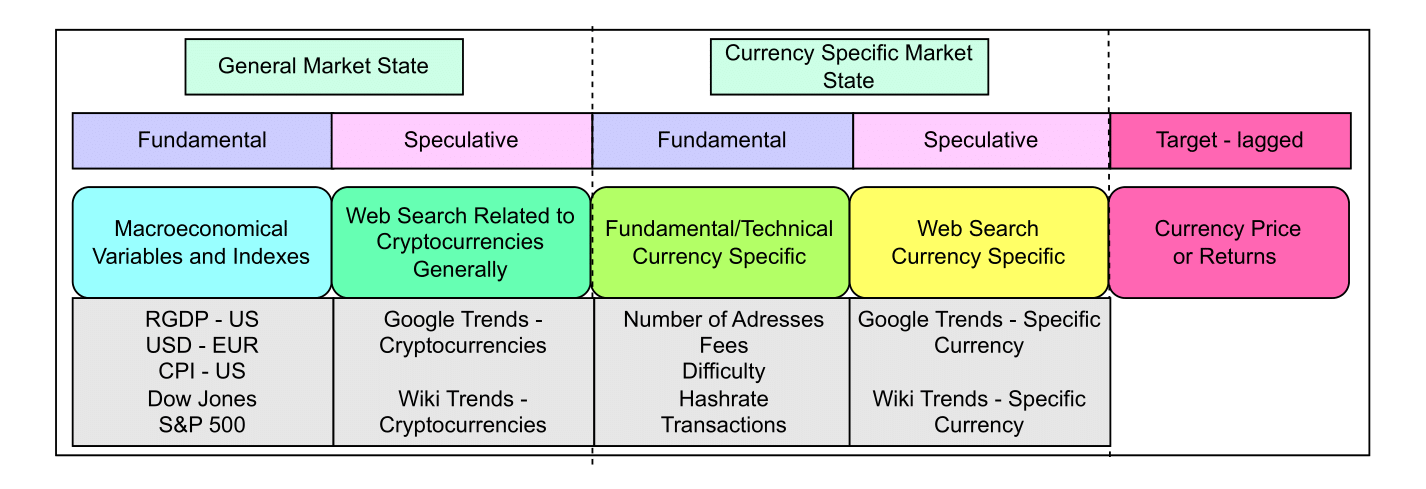
\includegraphics[width=1\textwidth]{Figures/dataset_description.drawio.png}
    \caption*{Source: Author}    
    \label{fig:dataset_description}
\end{figure}


The data were collected between December 2023 to February 2024 varying 
based on
the different sources but they are further shortened to utilize the most
overlapping region between data sources for each unique cryptocurrency.
This results in a time series from 17.9.2014 to 20.1.2024 for Bitcoin, 4.2.2016
to 27.7.2022 for Ethereum and series from 17.9.2014 to 21.12.2023
for Litecoin. The shifted versions of the datasets are of variable length based
on the forecasting horizon. 
\section{Cryptocurrency Specific Technical Data}

Despite the fact, that we have framed this data as fundamental/technical 
we should acknowledge that fundamental in our case stands far from its 
traditional meaning. They are fundamental in a way that they 
are the typical data researchers and practitioners employ to model cryptocurrencies
and that they objectively describe the system.
However, as the fundamental factor is very limited in this case it only makes sense
for the typical variables such as capitalization, volatility, hashrate and others.
But we also used a lot of technical variables that are derived from these fundamental
variables or the price itself. These help to identify trends in certain 
variables from pure mathematical transformation of the original series. 
All of these data were collected from \textbf{\href{https://coinmetrics.io/}{coinmetrics.io}}
and further processed by our pipeline.


We incorporate many variables describing specific technical characteristics of the network. Starting with number of active addresses
which acts as a measure of user activity on a particular day that is a cruical parameter potentially capturing the strength of 
bull or bear market behaviour. However, it does not reflect the direction itself. The difficulty of the network is
adjusted dynamically to counteract the changes in the mining power and thus act as a proxy for current mining power of the network or the current efforts of the miners. 
The size of the block is another characteristic of the network describing the size of the block (in bytes) and has been steadily increasing overtime
with significant fluctuation that depend on many other changes in the network. Hashrate is a measure of how
fast do the miners solve the hash for one block. In the long term the mean hashrate should be proportional to the difficulty at least that is how the 
\ac{BTC} protocol was designed however there are some fluctuation in the short term as the difficulty is adjusted every 2016 blocks 
to match the average hashrate over that period.


Other variables focus on the economics of the currency and model the market behaviour not the network itself. 
Beginning with traditional market signals such as capitalization indicating the overall price of all coins and volatility of returns 
as a standart deviation of log-returns. Furthermore, we employ many other variables about the price of fees 
provided by the users, revenues of the miners, distribution of wealth in the network and the number of transactions for that interval.


For the full description of the variables for \ac{BTC} please refer to the Appendix~\ref{app:var_desc}.


The datasets for Ethereum and Litecoin look similar with the exception of a few variables missing,
please see (\ref{litecoin:missing}):

    \begin{figure}[!htbp]
        \begin{center}
        \caption{Litecoin missing variables}\label{litecoin:missing}
        \begin{boxeditemize}
            \item \textit{Flow, in, to exchanges, USD}
            \item \textit{Flow, out, from exchanges, USD}
            \item \textit{Revenue, per hash unit, USD}
        \end{boxeditemize}
        \end{center}
        \end{figure}


\section{Macroeconomical Data}

As the macroeconomical condition is a cruical factor for investor behaviour 
we decided to include relevant variables that might deliver valuable
insights. We utilize five macroeconomical indicators that affect invesment choices.
Real Gross Domestic product of the United States represents the overall
growth trend of the largest economy in the world with closely related real
gross domestic product per capita telling more about individual resouces which
gives a more complex picture of the state of the US economy despite the 
fact that americans are not the main cryptocurrency investors by nation.
Furthermore we incorporate Consumer Price Index in the United States that
acts as an inflationary measure to capture the spurious correlation between 
prices of USD and BTC-USD exchange rate. M2 base acts as a measure
of dollar liquidity in the circulation. Lastly, the USD-EUR exchange rate
can be thought of as a market state information or its returns as an 
opportunity costs for potential investors. To further adress the problem of spurious
correlation and add the information about growth of other markets we include
various closing prices and other measures of the stock market and other 
investment opportunities. 


For the full description of 
the variables please refer to Table~\ref{tab:variables_macro}.

\begin{table}[htbp]
    \centering
    \begin{threeparttable}
    \caption{Macro Variables Descriptions}
    \label{tab:variables_macro}
    \begin{tabular}{ll}
    \toprule
    \textbf{Variable} & \textbf{Description} \\
    \midrule
    \texttt{Close\_DJI} & Dow Jones Industrial Average \\
    \texttt{Close\_GSPC} & S\&P 500 \\
    \texttt{Close\_GC=F} & Gold Futures \\
    \texttt{Close\_VIX} & CBOE Volatility Index \\
    \texttt{Close\_IXIC} & NASDAQ Composite \\
    \texttt{Close\_SMH} & VanEck Semiconductor ETF \\
    \texttt{Close\_VGT} & Vanguard Information Technology Index Fund \\
    \texttt{Close\_XSD} & SPDR S\&P Semiconductor ETF \\
    \texttt{Close\_IYW} & iShares U.S. Technology ETF \\
    \texttt{Close\_FTEC} & Fidelity MSCI Information Technology Index ETF \\
    \texttt{Close\_IGV} & iShares Expanded Tech-Software Sector ETF \\
    \texttt{Close\_QQQ} & Invesco QQQ Trust \\
    \texttt{RGDP\_US} & Real Gross Domestic Product of the United States \\
    \texttt{RGDP\_PC\_US} & Real Gross Domestic Product per capita 
    of the United States \\
    \texttt{CPI\_US} & Consumer Price Index: All Items: Total for United States \\
    \texttt{M2\_US} & M2 Base US \\
    \texttt{USD\_EUR\_rate} & U.S. Dollars to Euro Spot Exchange Rate \\
    \bottomrule
    \end{tabular}
    \end{threeparttable}
\end{table}

\section{Web Search Data}

As mentioned earlier following many other researchers we aimed to 
obtain a proxy for the market
attention. We specifically used \textbf{\href{https://pageviews.wmcloud.org/}{Wikipedia Page Views}}
to get the page views for Wikipedia pages: Bitcoin, Ethereum, Litecoin and 
Cryptocurrency and use them respectively for each coin dataset combining 
the overall Cryptocurrency views with the specific currency. Similarly we 
hoped to obtain similar data from 
\textbf{\href{https://trends.google.com/trends/}{Google Trends}} but they
turned out to be quite cumbersome to use. As \cite{West2020a} mentioned 
there are three main obstacles when using Google Trends. Firstly, the scale
is always normalized into the range 0-100 based on the selected region and time.
Secondly, this implicitly means that the results are rounded to integers and thus 
loosing a lot of precision. Lastly, there is a limit of 5 queries that you can 
use at a time. This not only means that you cannot compare more search terms 
but it also means that when there are over five variations how the term might
be searched for one cannot do that effectively. Another problem, 
that we faced is that the data can be obtained only in weekly granularity
for longer periods and thus needs to be interpolated to daily which 
most likely sacrifices a lot of interesting dynamics on the daily level which
is significant regarding the volatility of cryptocurrencies. 
These reasons, except the weekly sampling frequency, were solved in 
the \textbf{\href{https://github.com/epfl-dlab/GoogleTrendsAnchorBank}{g-tab}}
Python library, created by \citep{West2020a}, which uses a 
two step query sampling process that 
estimates the searches on a universally common scale with floating precision and allows 
us to use as many word formulation as needed. We would then sum the popularity
for each word formulation that is related to the same thing. We acknowledge
that there is a risk that we ommited some word formulations but hopefully
we covered all the significant ones.


Following is the list of the variables from this section and their word forms
for Google Trends:

\begin{table}[htbp]
    \centering
    \begin{threeparttable}
    \caption{Search Variables Descriptions}
    \label{tab:variables_search}
    \begin{tabular}{ll}
    \toprule
    \textbf{Variable} & \textbf{Description} \\
    \midrule
    \texttt{Wiki\_btc\_search} & Wiki pageviews for \textbf{\href{https://cs.wikipedia.org/wiki/Bitcoin}{Bitcoin}} \\
    \texttt{Wiki\_eth\_search} & Wiki pageviews for \textbf{\href{https://cs.wikipedia.org/wiki/Ethereum}{Ethereum}} \\
    \texttt{Wiki\_ltc\_search} & Wiki pageviews for \textbf{\href{https://cs.wikipedia.org/wiki/Litecoin}{Litecoin}} \\
    \texttt{Wiki\_crypto\_search} & Wiki pageviews for \textbf{\href{https://en.wikipedia.org/wiki/Cryptocurrency}{Cryptocurrency}} \\
    \texttt{Google\_btc\_search} & Google Trends summed across terms:  \\ & \textit{Bitcoin, bitcoin, BTC} \\
    \texttt{Google\_eth\_search} & Google Trends summed across terms:  \\ & \textit{Ethereum, ethereum, ether, ETH} \\
    \texttt{Google\_ltc\_search} & Google Trends summed across terms:  \\ & \textit{Litecoin, litecoin, LTC} \\
    \texttt{Google\_crypto\_search} & Google Trends summed across terms: \\ & \textit{Cryptocurrency, cryptocurrency, Cryptocurrencies}, \\ & \textit{cryptocurrencies, crypto, Crypto} \\
    \bottomrule
    \end{tabular}
    \end{threeparttable}
\end{table}


\section{Preprocessing}


Forecasting from historical data comes with many identified challenges. These
were especially pronounced in our case as we incorporate data from many
different sources with different sampling frequencies. Despite the fact
that our focus is on forecasting daily price and returns we use data
that come in weekly and monthly frequencies. We suggest two general concerns 
with such data. As we are using historical explanatory variables
to predict a response variable in the future we need to ensure that our
explanatory variables are already published at the time of forecasting and not
use data from the future. We implement forward filling after the data is resampled
to daily frequencies as a remedy. Especially for the macroeconomical data
we implicitly match those indicators to future dates that they do not trully
corespond to. Concretely, the Consumer Price Index for January is published at the 
beginning of February but as we forward fill this variable the Consumer Price Index
from January will actually be in February. This ensures that when we are 
forecasting with a 10 day horizon at the beginning of February we only use
data that was present at that time. The second concern is the fact 
that there is a lot of lost signal during those interpolated periods 
and the daily dynamics are not incorporated in the model. Unfortunately,
this is the nature of economic research as especially the 
macroeconomical indicators come typically in such sampling frequencies.
As already suggested these preprocessing steps were applied to the macroeconomical
indicators, Google Trends that come in weekly frequency and for 
ETFs and indexes that are not traded on the weekends, see Figure~\ref{fig:dataset_interpolation}.

\begin{figure}[!h]
    \centering
    \caption{Resampling data to daily frequency is implemented
    using forward filling to avoid future distribution leakage.}
    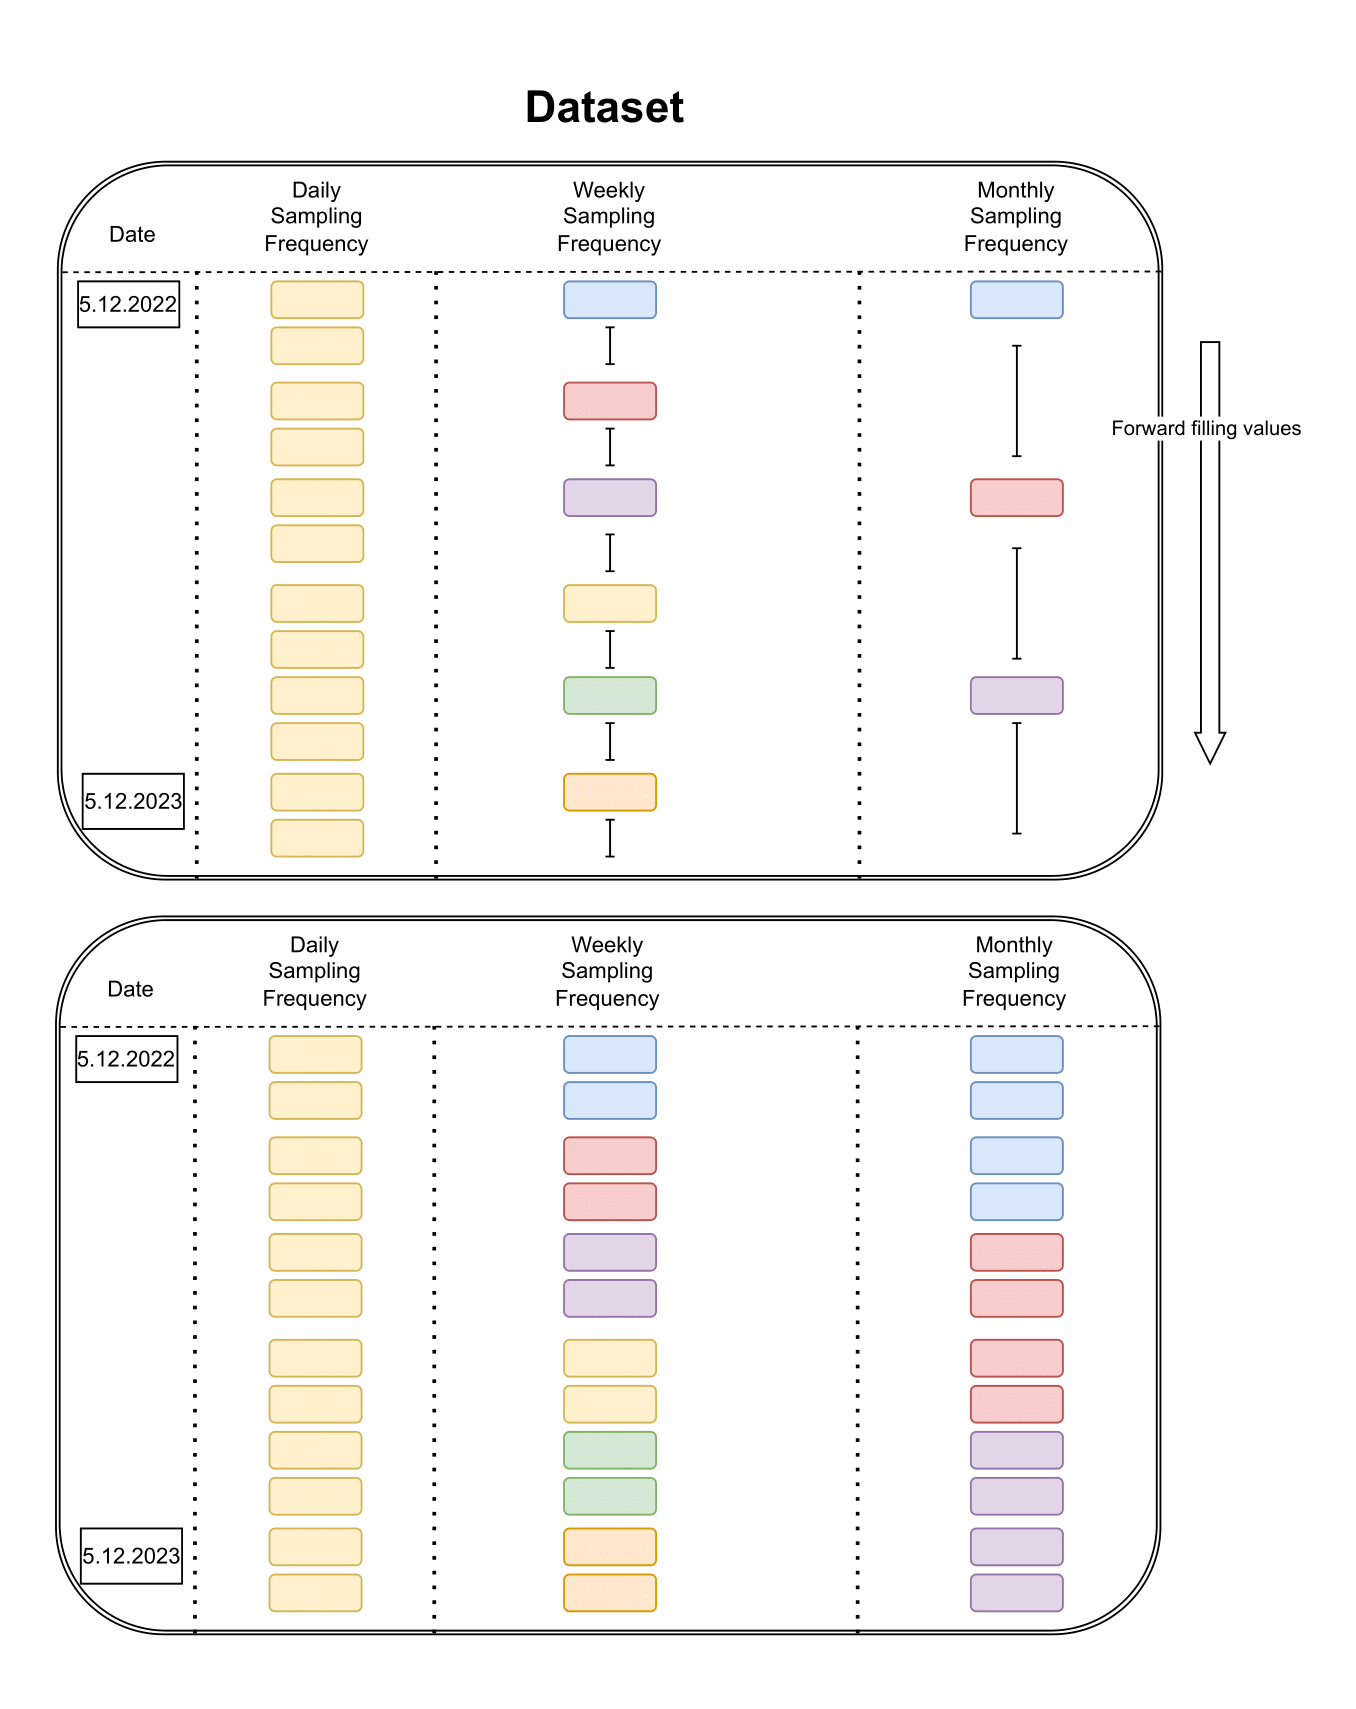
\includegraphics[width=1\textwidth]{Figures/data_interpolation.drawio.png}
    \caption*{Source: Author}    
    \label{fig:dataset_interpolation}
\end{figure}

As some of the variables are missing at the beginning of the time frame there
is no clear solution how to impute them without leaking the future distribution.
Even though we could say that this rule might be violated on the training set
but we opted for a different approach.
We start by visually inspecting the structure of the missing values and 
set the start of the series as such that "almost all" variables are already 
being collected. The aim is to keep as much data as possible but avoid
having a lot of data points at the beginning with different distribution changed 
by imputation. After that we fill the data that is missing only at the start with
zeros in order to avoid imputing future data. There is also a second reason
as generaly these variables are increasing and thus imputing zeros makes 
even mathematical sense. Especially for data like Googe Trends or Wikipedia
Pageviews this is a reasonable imputation. Finally we cut the 
\ac{ETH} series at the switch to proof-of-stake as this completely
changes the modeling perspective and we merge all the data
from different sources on the date column.


The most cruical step is the transformation of this dataset into a supervised
learning problem. We will proceed with the example of BTC price, however
the same will hold for other coins and returns forecasting. We employ
forecasting with 1, 5 and 10 day horizon $h$. We denote the number 
of observations $\mathbf{x_{i}}$
as $n$ and the number of features $j$ as $k$.

\begin{equation}\label{eq:horizon}
    h \in \{1,5,10\}
\end{equation}
\begin{equation}\label{eq:features}
    j \in \{1,...,k\}
\end{equation}
\begin{equation}\label{eq:observations}
    i \in \{1,...,n\}
\end{equation}

We start by denoting
the original dataset $\mathbf{X} \in \mathbb{R}^{n \times k}$.
Now assuming $\mathbf{X}_{:,k} = [\mathbf{x}_{1k},...,\mathbf{x}_{nk}]$ 
is the \ac{BTC} price feature vector we shift it
back in time by $h$ and drop the data without corresponding counterpart. 
Concretely, we drop all 
$\mathbf{X}_{n-h:n,1:k-1}$ and $\mathbf{X}_{1:h,k}$.
With this technique we always sacrifice $2h$ observations from the original dataset.
If we further split the dataset into the explanatory and target features
and reset the indexation such that we denote $m = n-2h$
we end up with the following matrices where the target matrix Y is essentially
only a vector where $y^\top = \mathbf{X}_{:,k}$, see Figure~\ref{fig:dataset_shift}.

\begin{figure}[!h]
    \centering
    \caption{Transforming data into supervised learning problem
    by shifting target variable by the forecast horizon back in time.}
        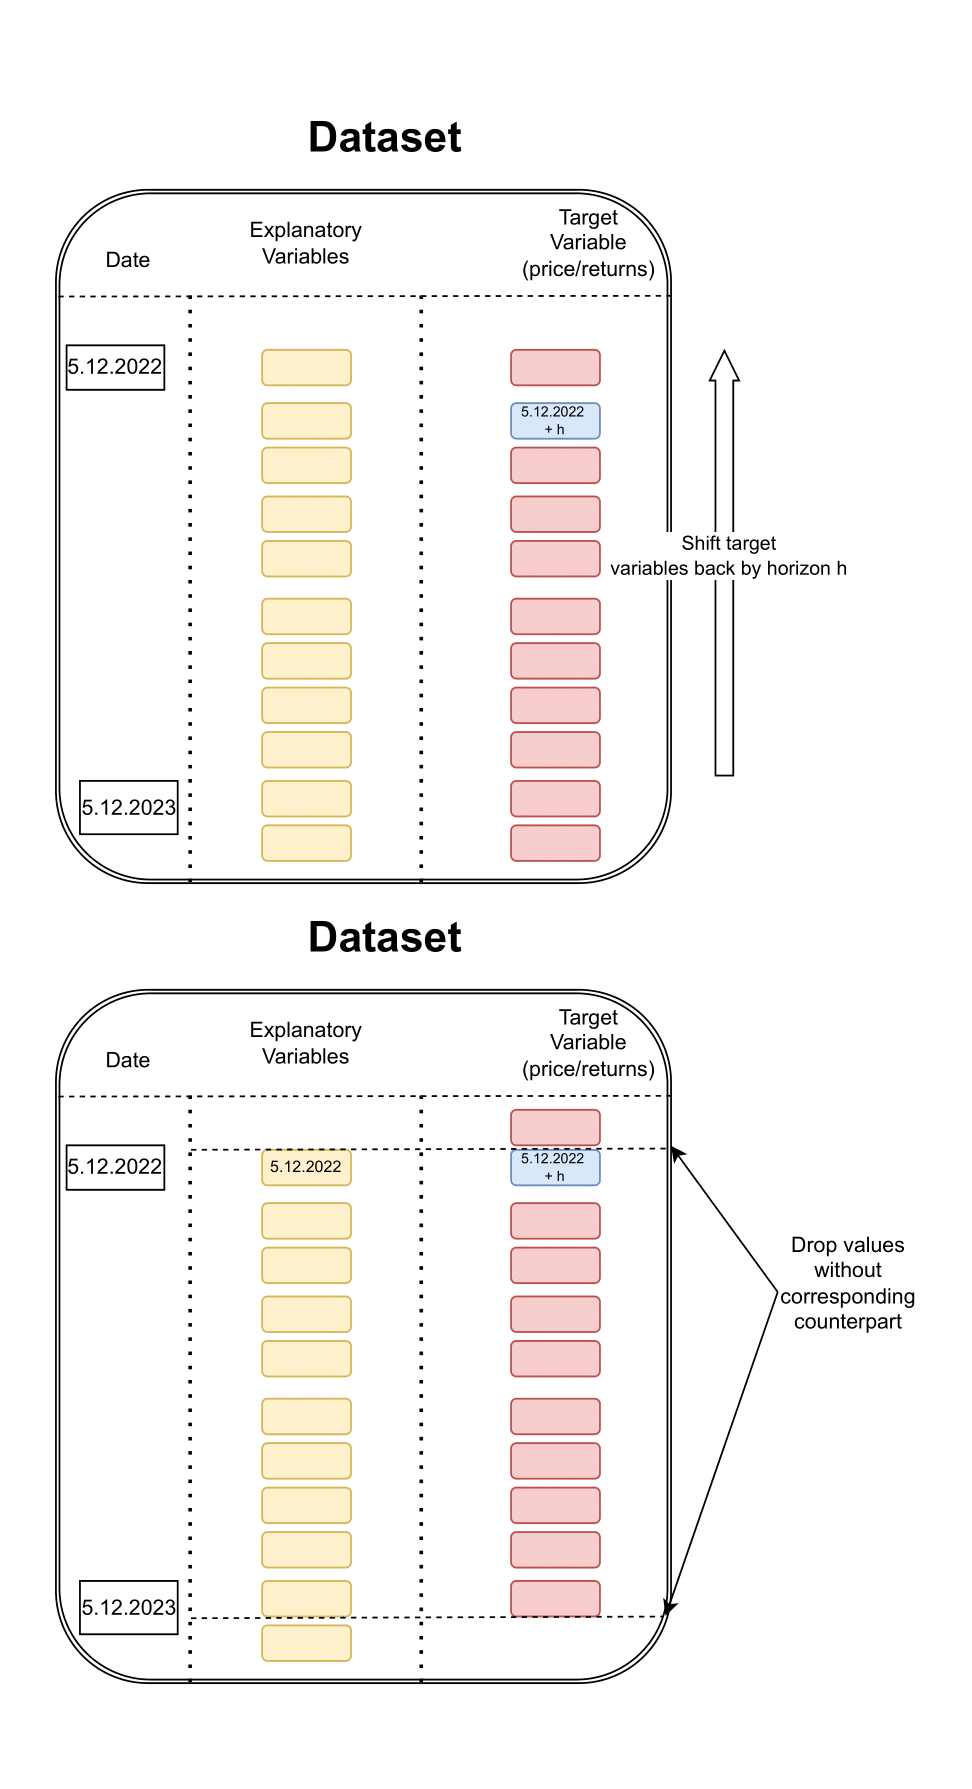
\includegraphics[width=1\textwidth, height=0.9\textheight,keepaspectratio]{Figures/data_shift.drawio.png}
    \caption*{Source: Author}
    \label{fig:dataset_shift}
\end{figure}

\begin{equation}\label{eq:explanatory}
    \mathbf{X} \in \mathbb{R}^{m \times {k-1}} = 
    \begin{pmatrix}
        x_{11} & x_{12} & \dots  & x_{1k-1} \\
        x_{21} & x_{22} & \dots  & x_{2k-1} \\
        \vdots & \vdots & \ddots & \vdots \\
        x_{m1} & x_{m2} & \dots  & x_{mk-1}
    \end{pmatrix}
\end{equation}

\begin{equation}\label{eq:target}
    \mathbf{Y} \in \mathbb{R}^{m \times 1} = \mathbf{y^\top} = 
\begin{pmatrix}
    y_{1}\\
    y_{2}\\
    \vdots  \\
    y_{m} 
\end{pmatrix}
\end{equation}
We can now observe that modeling $y_i$ as a function of
explanatory variables $x_{i}$ is a forecasting with horizon $h$ into the future.
Where we essentially try to estimate the function $f_{foreacast}$.
\begin{equation}\label{eq:model_simple}
    y_i = f_{forecast}(\mathbf{x}_{i})
\end{equation}

The final preprocessing step is specific to the \ac{LSTM} network which is
a type of architecture that requires the input to be of 
the shape (num timesteps, num features).
This means that it can use for example 10 day history for each variable
and forecast the target variable. This is a really strong feature and 
makes it a viable option for our usecase. In order to use it, the input dataset
has to be reshaped in such a way that for observation $\mathbf{x_{i}}$ 
concatenates values from $\mathbf{x}_{i}$ 
up to $\mathbf{x}_{i-lag}$, see Figure~\ref{fig:dataset_lstm_reshape}


\begin{equation}\label{eq:lstm_reshape}
    \mathbf{X}_{i,:} = [[{x}_{i1},...,{x}_{ik}],
    [{x}_{i-11},...,{x}_{i-1k}],
    [{x}_{i-lag1},...,{x}_{i-lagk}],...]
\end{equation}

\begin{figure}[!h]
    \centering
    \caption{Reshaping for LSTM network requires applying
    sliding window over the whole dataset to introduce temporal information
    to the model.}
    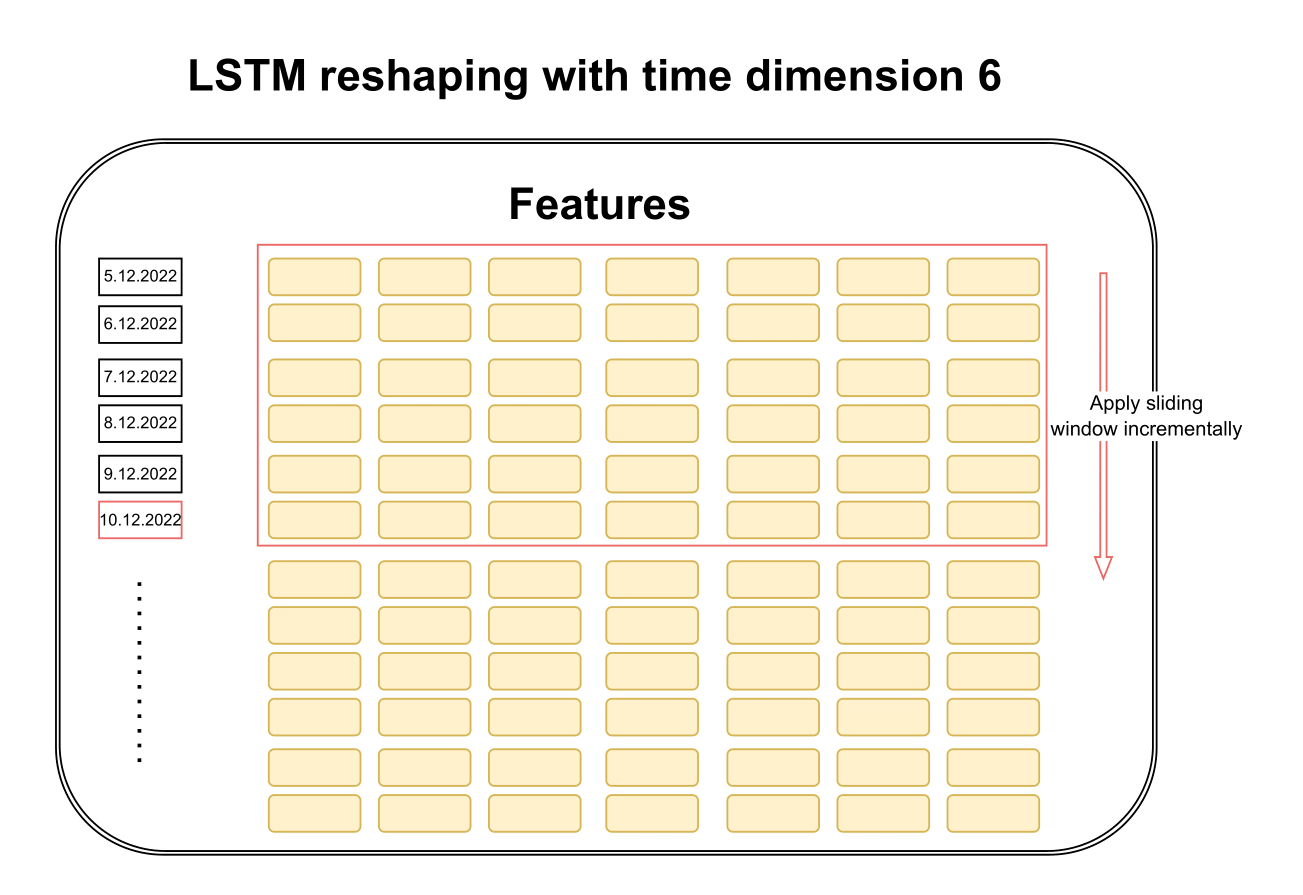
\includegraphics[width=1\textwidth]{Figures/LSTM_reshaping.drawio.png}
    \caption*{Source: Author}
    \label{fig:dataset_lstm_reshape}
\end{figure}
\chapter{Methodology}
\label{chap:four}

\section{\acl{ML}}

It is generally agreed upon that the term 
\ac{ML} refers to the field of study that gives computers the ability to learn 
without being explicitly programmed. This fact was first 
introduced by Arthur Samuel in 1959 \cite{Samuel1959}. However, note that the reference to this paper is used
loosely, as the term \ac{ML} was not directly used in the paper and it is rather 
a retrospective interpretation of the paper. 

The term \ac{ML} was more explicitly introduced by Tom M. Mitchell in 1997 \cite{Mitchell1997}:

\begin{defin}[Machine Learning]\label{de:ml}
    A computer program is said to learn from experience E with respect
    to some class of tasks T and performance measure P, if its performance at tasks in
    T, as measured by P, improves with experience E. 
\end{defin}

Typically, the experience E is represented by a dataset, which is used to train the model. 
We can generally say that \ac{ML} is the ability to get better at specified task by learning
from provided relevant data without problem domain specific programming of the computer.


Nowadays \ac{ML} is at the core of many applications that we use daily. The usecases range from
spam filters, recommendation systems, medical diagnosis, stock trading, and many more. Currently, 
machine learning is dominated by deep learning, which is a subfield of \ac{ML} that focuses on
deep neural networks that rely on large datasets in order to be able to generalize well.
On the other, hand traditional \ac{ML} algorithms are still widely used and are often the first choice
when the dataset is small or the problem is low dimensional. Whereas deep learning models
can be used in high frequency data, where the datasets are large enough to train the model, 
daily closing stock price prediction is a task that can be successfully solved with 
traditional \ac{ML} algorithms. As the datasets are much smaller. 


In general, cryptocurrencies
lie somewhere in the middle of the spectrum. Exactly as stocks, either high frequency or low frequency
data can be chosen based on the research question. The difference however is that cryptocurrencies 
are much more volatile than stocks, and they can have much higher dimensionality as we can use 
many technical analysis indicators to predict the price. 
That is why we will use a combination of
traditional \ac{ML} algorithms and deep learning models to predict the 
closing prices or returns of
various cryptocurrencies.

\ac{ML} algorithms can be divided into three main categories: supervised learning, unsupervised learning, and reinforcement learning.
As mentioned earlier, we will focus on supervised learning as the process of forecasting
can be easily transformed into a supervised learning problem where the input features
are historical or current data and the output is the future price or return.


It is important to note on the fundamental difference between machine learning and
traditional econometric models. In econometrics the focus is to uncover the underlying
relationship between the variables and to understand the size of contribution of each
feature. In machine learning, the focus is mainly on maximizing the performance metric for predictions and 
the magnitude of the effects usually remains unknown. This is definitely a weakness of machine learning
which researchers try to adress by developing new field of explainable \ac{AI}. 
Where they focus on developing models that are able to explain their predictions in a human understandable way.
They provide a significant promise for the use of \ac{ML} methods in finance in the future
where the interpretability of the model is crucial for customers or regulators in specific subfields.





\section{Ridge Linear Regression}
The simplest model that we can use for forecasting is the \acl{LR} model.
Generally, there exists a closed form solution for the \ac{LR} model.

\begin{equation}
    \hat{y} = \theta_0 + \theta_1 x_1 + \theta_2 x_2 + \cdots + \theta_n x_n
\end{equation}

But in practice, we use gradient descent to find the optimal parameters.
Gradient descent is an optimization algorithm used to minimize the cost
function provided to the model. The idea is that we compute
partial derivation of the error function with respect to each parameter
of the model and update the parameters in the opposite direction of the gradient
where the learning rate is the step size of the update. Usually, 
minibatch gradient descent is used where the gradient is averaged over a small
batch of randomly sampled data.

The update rule for the parameters \(\theta\) using gradient descent is given by:

\begin{equation}
    \theta_j := \theta_j - \alpha \frac{\partial J(\theta)}{\partial \theta_j}
\end{equation}

where \(\alpha\) is the learning rate and \(J(\theta)\) is the cost function.
We have decided to use linear regression as a model representing 
the class of simple linear models. However, even though the model is simple,
it can still suffer from overfitting the training data. There exists
a relatively straight forward solution to this problem called Ridge regression.
Ridge regression is a linear regression model with a regularization term added to the cost function
which penalizes the model for having large weights. 

The cost function for Ridge regression is given by:

\begin{equation}
    J(\theta) = \text{MSE}(\theta) + \frac{\lambda}{2} \sum_{j=1}^{n} \theta_j^2
\end{equation}

where \( \lambda \) is the regularization parameter. Note that the bias term \(\theta_0\) is not regularized
and that the regularization term is used only during training.


\section{Support Vector Machines}

Support Vector Machines are widely used \ac{ML} algorithm which was expected to 
be the future of machine learning in the early 2000s. However, the rise of deep learning
has overshadowed the success of \ac{SVM}s. Nevertheless, \ac{SVM}s are still widely used
as they are really useful for small datasets and can capture complex nonlinear relationships.

To ilustrate the idea of \ac{SVM}s, let us consider a binary classification problem.

\begin{figure}[!h]
    \centering
    \caption{Support Vector Machines}
        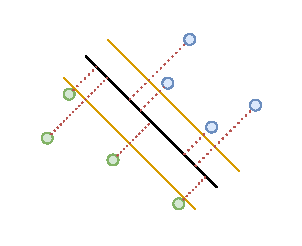
\includegraphics[width=1\textwidth]{Figures/SVM_idea.drawio.pdf}
    \label{fig:svm}
\end{figure}


The idea is to find the hyperplane that maximizes the margin between the two classes.
This implies that the hyperplane actually depends only on the support vectors which are the points
closest to the hyperplane. This can be relatively easily reformulated
into a regression problem by using the same idea but instead of classifying the points
we are predicting the distance from the hyperplane. This is called the support vector regression.
Note that the example in Figure \ref{fig:svm} represents a problem that is linearly separable
which is often not the case in practice and there are two remedies how to fix that.
The first one is the usage of the kernel trick which is a way to transform the data into a higher dimensional space
where the data is linearly separable. The second one is to use the \ac{SVM} with a soft margin which is
what most of the \ac{SVM} implementations do. That allows us to set a hyperparameter that allows
some points to be missclasified and acts as a form of regularization where we do not perfectly,
seperate all of the points in the training set. 


The optimization details of the \ac{SVM}s are quite complex and are beyond the scope of this text.
They include the usage of the Lagrange multipliers and the dual optimization problem. The description
of the kernel trick is not included as we opted for the linear kernel in our experiments.
We thus refer the readers to some traditional \ac{ML} textbooks such as \cite{bishop2006pattern}.
The \ac{SVM}s represent a middle ground between the traditional \ac{LR} model and the deep learning models.


\section{\acl{LSTM} \acl{RNN}s}

\section{\acl{PCA}}

\ac{PCA} is a widely used dimensionality reduction technique that is able
to reduce number of dimensions for the purpouses of visualization, noise reduction, and
reduction of the curse of dimensionality. The curse of 
dimensionality referts to the fact that with increasing number of 
dimensions the volume of the space increases exponentially and the data points become
extremely sparse leading to enormous distances between training points.
The fact that \ac{PCA} can be used as a noise reduction technique is 
technically a byproduct of the way how this algorithm works. We will start with the
general idea to ilustrate how this concept emerges.


Conceptually, \ac{PCA} can be thought of in two ways: maximum variance formulation
and minimum reconstruction error formulation. We will follow with the maximum variance formulation.
The idea is to find the hyperplane that maximizes the variance of the data projected onto it.
Refer to Figure \ref{fig:pca} for the illustration of the concept. We can see
that the first principal component is the line that maximizes the variance of the projection
of the data onto it. The second principal component captures
less variance and is orthogonal to the first principal component. \ac{PCA} can
generally create as many principal components as there are dimensions in the data.
This means that for \textit{n} dimensions we can create \textit{n} principal components which
are orthogonal to each other and are odered by the amount of variance they capture. 
Finally we can reduce the number of dimensions by projecting the data onto the first \textit{k} principal components
where \textit{k} is the number of dimensions we want to keep or the desired variance 
we want to preserve.

\begin{figure}[!h]
    \centering
    \caption{\ac{PCA} Hyperplanes}
        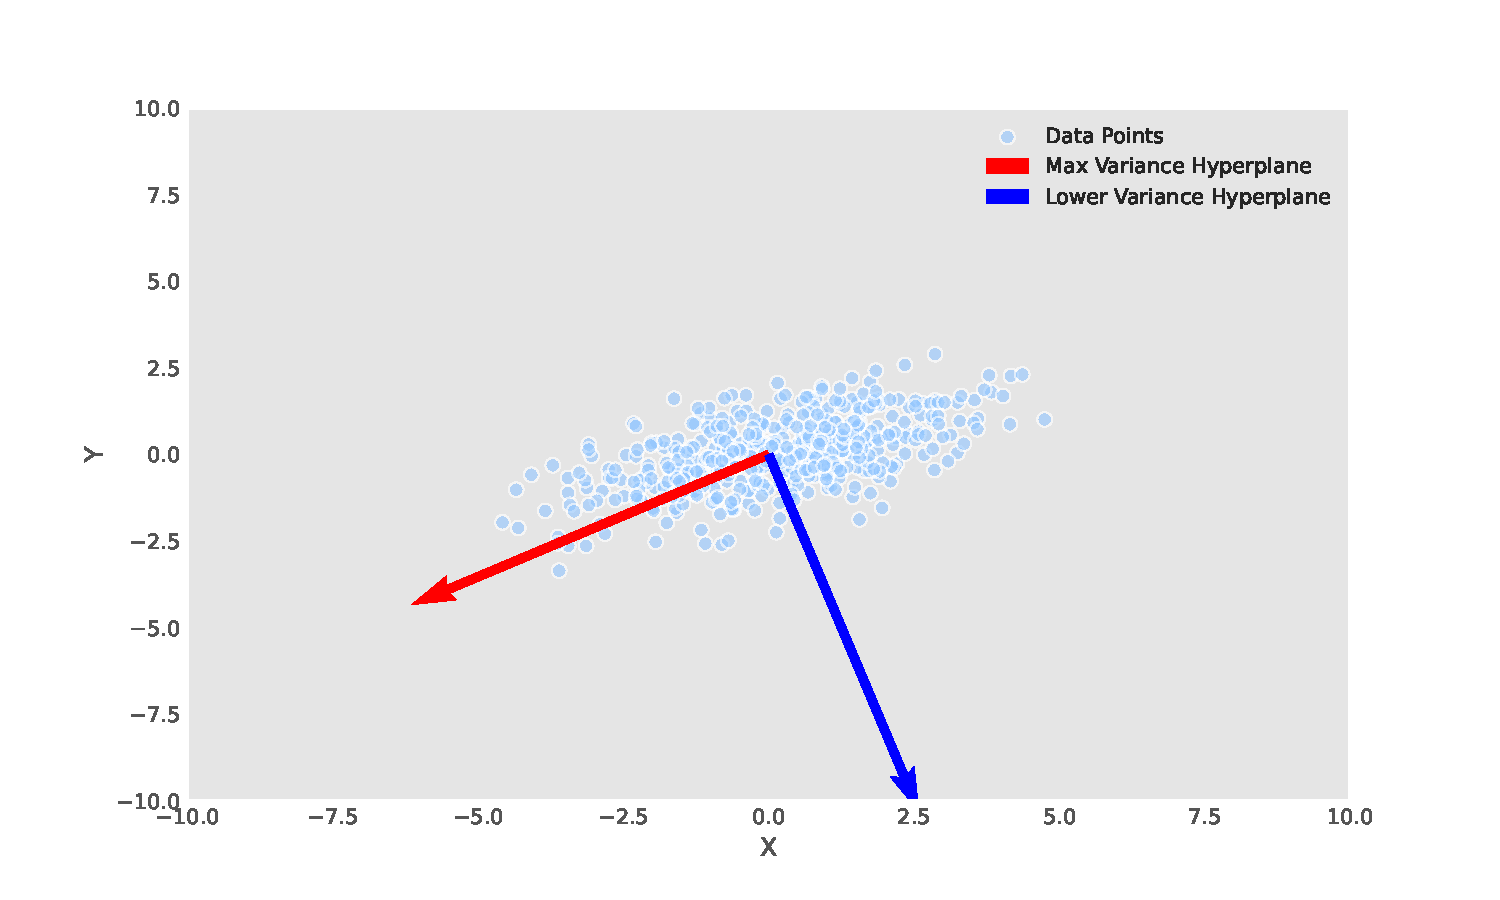
\includegraphics[width=1\textwidth]{Figures/pca_plot.pdf}
    \label{fig:pca}
\end{figure}

This is where the idea that \ac{PCA} can be used as a noise reduction technique comes from.
As this algorithm keeps only data which captures most of the variance
and theoretically should drop information that is less informative.
It is interesting to note that as the principal components are orthogonal to each other 
they are also uncorrleated which is a useful property for many \ac{ML} algorithms. 
We acknowledge that \ac{PCA} is not in itself a noise reduction technique
but it is a rather elegant and simple way that sometimes reduces noise in the data.
The implementation details of \ac{PCA} are beyond the scope of this text but we refer the readers
to the original paper by Pearson \cite{Pearson1901}.




\section{Stationarity in Time-Series}

We would like to explicitly adress the concept of stationarity as there 
seems to be a lot of confusion around the topic especially because the boundary between 
traditional econometric models and machine learning models is not always clear.

Stationarity is a crucial concept in time-series analysis. Despite the fact, that there exist
many tests and rigid definitions for it, it is often reduced to the 
concept of constant mean and variance or generally to the fact that the parameters
of the distribution do not change in time. Without this property the errors
of the model become function of time which is not desirable for proper inference.

Econometrics usually prefers stationary data for aforementioned reasons because it 
is cruicial for inference and interpretation of the results. That is 
why econometricians like to model returns instead of prices, as returns
should generally be stationary. Imporantly, there is always the possibility
to transform the predictions back to the original prices by adding the forecasted
returns to the last observed price and potentially reversing some normalization steps.

This is different for \ac{ML} as the focus is on prediction and the models are fundamentally 
different. As the models are trained using gradient descent and not using the
analytical solutions, the stationarity is not as crucial. Clearly, 
the models will perform better on stationary data because it requiers much 
less capacity for the model as some of the information removed by differencing.
However, models with enough capacity can easily learn non-stationary data and
capture information about trends, seasonalities, and other patterns. 
Thus we decided to test our models on both prices directly and on returns where
the results are much less dependent on changes in the distribution of the data.

\section{Proposed Forecasting Framework}

We propose a forecasting framework which is designed to compare the performance between using \ac{PCA} as a 
dimensionality reduction technique and using the raw data. 
The framework is shown in Figure \ref{fig:forecasting_framework}.
The preprocessing layer is responsible for cleaning the data, filling in missing values and tranforming 
the problem to supervised learning as described 
in \ref{chap:three}. Following stage is responsible for reducing the number of features. 
The first \ac{PCA} step transforms the data onto \textit{n} principal components and the filtering step
chooses the most important features such that their cumulative variance adds up to 95\%, 98\% or 99\%.
As decreasing the dimensionality would completely change the desired
complexity of the algorithms and the differences might be attributed only to the change 
of dimensionality we upsample the data back to the original dimensionality using 
the inverse transformation of the \ac{PCA} algorithm.

Following is the \ac{LSTM} reshaping layer that is responsible for transforming the data into a 3D tensor for 
the \ac{LSTM} \ac{RNN} as described 
in \ref{chap:three}. The most crucial layer is the forecasting layer that essentially consists of 3 parts.
Firstly, it normalizes the variables using robust scaler to ensure that the input features come from 
the same value range. Secondly, it uses grid search to search for the best
hyperparameters for the model. 
Lastly, it trains the model and evaluates the performance using the best found model. This is the reason
why we abstract the metrics layer seperately to make it apparent that the metrics are calculated
on the best model found by the grid search. The metrics layer is also the layer where
we can statistically compare the significance of the difference between the models.
It is important to note that this framework is executed across all specified forecasting models, 
cryptocurrencies of interest, and forecasting horizons as we expect the effects
to be quite different for different models and forecasting horizons. 


As we have already noted the fact that that the target price is clearly non-stationary,
has important implication for the choice of splitting strategy for the grid search 
hyperparameter optimization. 
There are two main strategies for splitting the data into training and testing sets.
The first one is traditional train, development, and test split where the model is trained on the training set,
hyperparameters are optimized on the development set, and the model is evaluated on the test set.
This approach is generally sufficient when the dataset is large enough and we believe
that the distributions of the three datasets are similar. 
A more robust approach is to use grid search with cross-validation. 
This approach makes sure that we have not overfitted the model to the development set.
Firstly, we split the data into training and testing set. And then 
we iteratively split the training set into training and validation set. 
Train the model on the training part of the train set and evaluate on the validation set.
Finally we average over the results across all validation sets and take the best hyperparameters
from the provided grid. This approach avoids overfitting and is typically
used when we have enough compute to train the models. 


Note that the goal of grid search is to create a robust representation of a 
reasonable test set distribution as it samples randomly the points into the training and validation set.
This approach works if the data is stationary and the distribution of the data does not change drastically in time.
But time series rarely have this property and cryptocurrencies suffer especially profound changes in the distribution
as they have grown in popularity. The difference between the training and test set
is extreme but that is something that we can do very little about as we want the test set
to be as close to the future as possible. 


Additionally, there is an extremely
common mistake that researchers make when they use grid search for time series data.
This problem is called data leakage and it occurs when future distribution of the data
is used to optimize the hyperparameters. As \ac{ML} models typically 
require data to be scaled and normalized, the parameters for the normalization 
need to be learned only on the historical data not on the future data otherwise the 
results will be biased and suggest higher quality of the model than it actually is.
Theoretically, this could be relaxed on the training set as the normalization
might be fitted on the whole training set but it is crucial that the test set distribution
is never leaked to the fitting procedure. However, we believe that
the correct methodology is to use a rolling window approach for the grid search
where the normalization parameters are fitted on the training set and the validation set.
This is why we use time series split for the grid search without randomly shuffling the data.
This approach splits the training set into \textit{k} folds and iteratively
trains the model on \textit{k-1} folds and evaluates on the \textit{k-th} fold.
This approach has the advantage that the model is actually trained with
different sized training sets which is useful for generalization properties
but has the disadvantage that the difficulty of the splits is extremely volatile.
This is definitely a limitation as the performances between splits
can vary significantly and averaging over the results might be prone to noise.
However, we believe that this is the methodologically correct approach.
\begin{figure}[!h]
    \centering
    \caption{Time Series Split with \textit{k=2}} 
        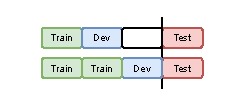
\includegraphics[width=1\textwidth]{Figures/time_series_split.drawio.pdf}
    \label{fig:ts_split}
\end{figure}
We opted to use only two splits as the the data size
is relatively small and the results were extremely noisy when using
more splits.


\begin{figure}[!h]
    \centering
    \caption{Proposed Forecasting Framework}
        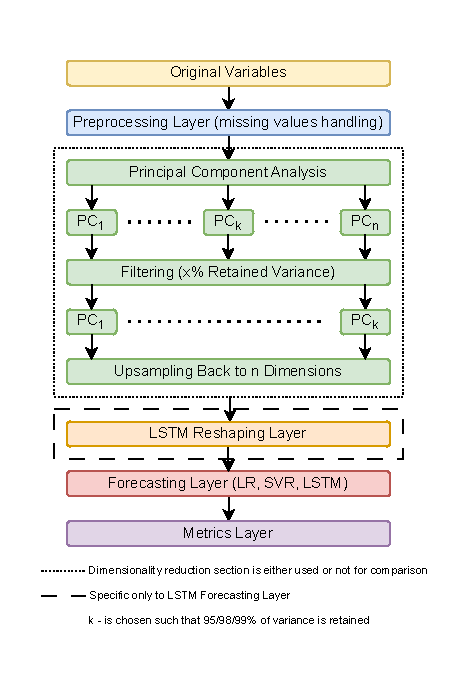
\includegraphics[width=1\textwidth]{Figures/Forecasting_framework.drawio.pdf}
    \label{fig:forecasting_framework}
\end{figure}
\chapter{Results and Discussion}
\label{chap:five}
In this section we will discuss the results obtained from 
the performed experiments. We particularly discuss the 
overfitting phenomenon, which is a common problem
for small sample sizes and for low signal to noise problems. 


\section{Results Intepretation}
\label{sec:results}
Initially, we intend to focus mainly on the price forecasting problem.
After running many experiments, we decided to add 
a set of technical indicators calculated from the price variable.
Concretely, we added the following indicators: simple moving average (SMA),
exponential moving average (EMA), relative strength index (RSI) and 
bollinger bands (BB). The reason for this decision is the fact
that the price variable is strongly autocorrelated and 
the fundamental pricing is relatively limited. 
To see the correlation matrix for the initial
dataset, see Figure \ref{fig:Corr_btc}.

\begin{figure}[!h]
    \centering
    \caption{Correlation matrix of the BTC dataset shows high level of 
    multicollinearity.}
    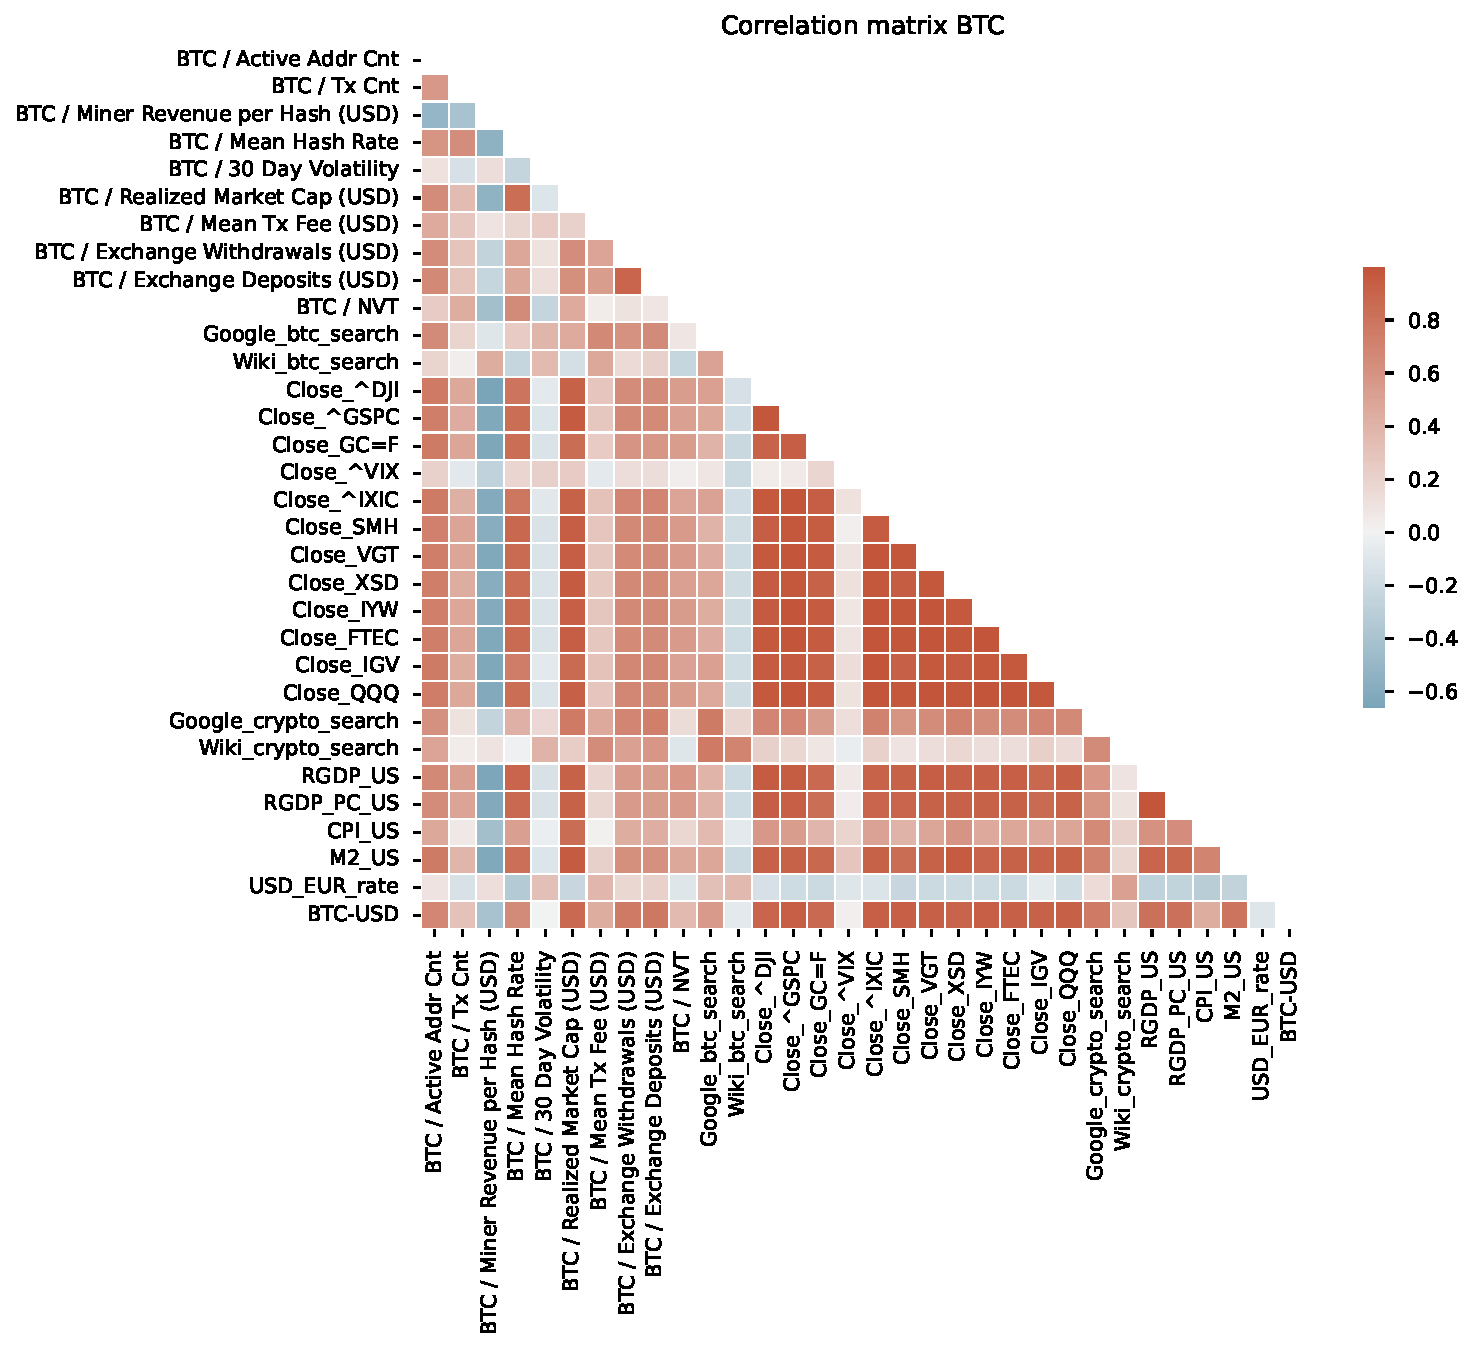
\includegraphics[width=1\textwidth]{Figures/Corr_btc.pdf}
    \caption*{Source: Author}
    \label{fig:Corr_btc}
\end{figure}

\begin{equation}\label{eq:sma}
    \text{SMA}_t = \frac{1}{w} \sum_{i=0}^{w-1} P_{t-i}
\end{equation}

\begin{equation}\label{eq:ema}
    \text{EMA}_t = \alpha P_t + (1 - \alpha) \text{EMA}_{t-1}, \quad \text{where} \quad \alpha = \frac{2}{w + 1}
\end{equation}

\begin{equation}\label{eq:rsi_avg}
    \text{AvgGain}_t = \frac{1}{w} \sum_{i=1}^{w} \max(\Delta P_{t-i}, 0), \quad
    \text{AvgLoss}_t = \frac{1}{w} \sum_{i=1}^{w} \max(-\Delta P_{t-i}, 0)
\end{equation}

\begin{equation}\label{eq:rsi}
    \text{RS}_t = \frac{\text{AvgGain}_t}{\text{AvgLoss}_t}, \quad
    \text{RSI}_t = 100 - \left( \frac{100}{1 + \text{RS}_t} \right)
\end{equation}

\begin{equation}\label{eq:bbands}
    \text{Upper}_t = \text{SMA}_t + k \cdot \sigma_t, \quad
    \text{Lower}_t = \text{SMA}_t - k \cdot \sigma_t
\end{equation}

After adding the technical indicators, the results
did not improve significantly and the model 
was always converging to the prediction of the current price
which leads to a typical pattern in the 
graph comparing the predicted and actual prices where the prediction
is the target price shifted by the time horizon.
We test this hypothesis by comparing
the model with the naive forecast which is the last
observed price and charaterizes
the random walk model. The naive forecast outperforms 
the model in most of the cases on the test dataset. 


In the following steps we decided to focus on the prediction
of log returns. The log returns are calculated as follows:
\begin{equation}\label{eq:log_returns}
    r_t = \log(P_{t+h}) - \log(P_t) = \log\left(\frac{P_{t+h}}{P_t}\right)
\end{equation}

where $P_t$ is the price at time $t$ and $h$ is the time horizon.
The idea behind this approach is that the log returns are stationary
and the model can better capture
the pricing dynamics without learning the long term trend.
Due to the fact that the log returns are stationary, 
$R^2$ is a good measure of the model performance that
tells whether the model is better than the naive mean forecast.
Positive $R^2$ indicates that the model is better than the naive forecast.
Unfortunately, this did not help much and the model was still
unable to generalize well to the test dataset despite
decent performance on the training dataset.


We suggest multiple reasons for this behavior. 
Either the signal to noise ratio is too low
and the model is not able 
to learn the pricing dynamics. 
The second reason is that the model is overfitting the training
data despite extremely strong regularization of many forms and despite
cross validation. We suspect
that the combination of the small sample size and the
nature of the cross validation 
are the main reasons for this behaviour. 

For time series data, the temporal ordering of the data is important.
That is the reason why one should not use the standard cross validation
in order to avoid data leakage especially 
for the scalers that scale the data into a range
which is required by some models. In practice, 
one can use normal cross validation on the training dataset
but it will most likely lead to overfitting.
The second option is to use the time series cross validation
which incrementally increases the training dataset 
and evaluates the model on the next batch of the data.
This approach is more robust but has its own limitations.
The first one is that when the sample size is small, 
the performance of the model is very noisy across the folds
which makes it difficult to evaluate the best hyperparameters. 
Furthermore, varying sample size actually 
leads to different number of gradient descent iterations
for some models which affects the choice of the best hyperparameters.
The second weakness is actually the reasons
that makes this approach more robust and that is the
act of masking the future distribution of the data.
As most machine learning models and certainly 
those used in our experiments including the \ac{PCA} step
expect the data to be standardized
or scaled to some predefined range.
When the distribution of the data changes
significantly, the scalers trained on the training dataset
will cause the test data to be scaled
outside of those expected ranges and thus breaking the 
performance of the model. 
Unfortunately,
this is the nature of our data 
and shows some limitations of the machine learning approach 
for problems that are changing over time.


Due to afforementioned problems, we opted for a different approach
which includes differencing and applying logarithm to all of
the independent variables to push them closer to stationarity.
This obviously leads to loss of information 
but may help with the cross validation problem.
Especially, variables that come in weekly and monthly frequencies
and are thus interpolated to daily frequency
will be zero most of the time and thus
may introduce a lot of variance on the edges where the values
are changing. For the correlation matrix of this transformed 
dataset see Figure \ref{fig:Corr_btc_logdiff}.

\begin{figure}[!h]
    \centering
    \caption{Correlation matrix of the BTC dataset after
    log differencing all of the variables.}
    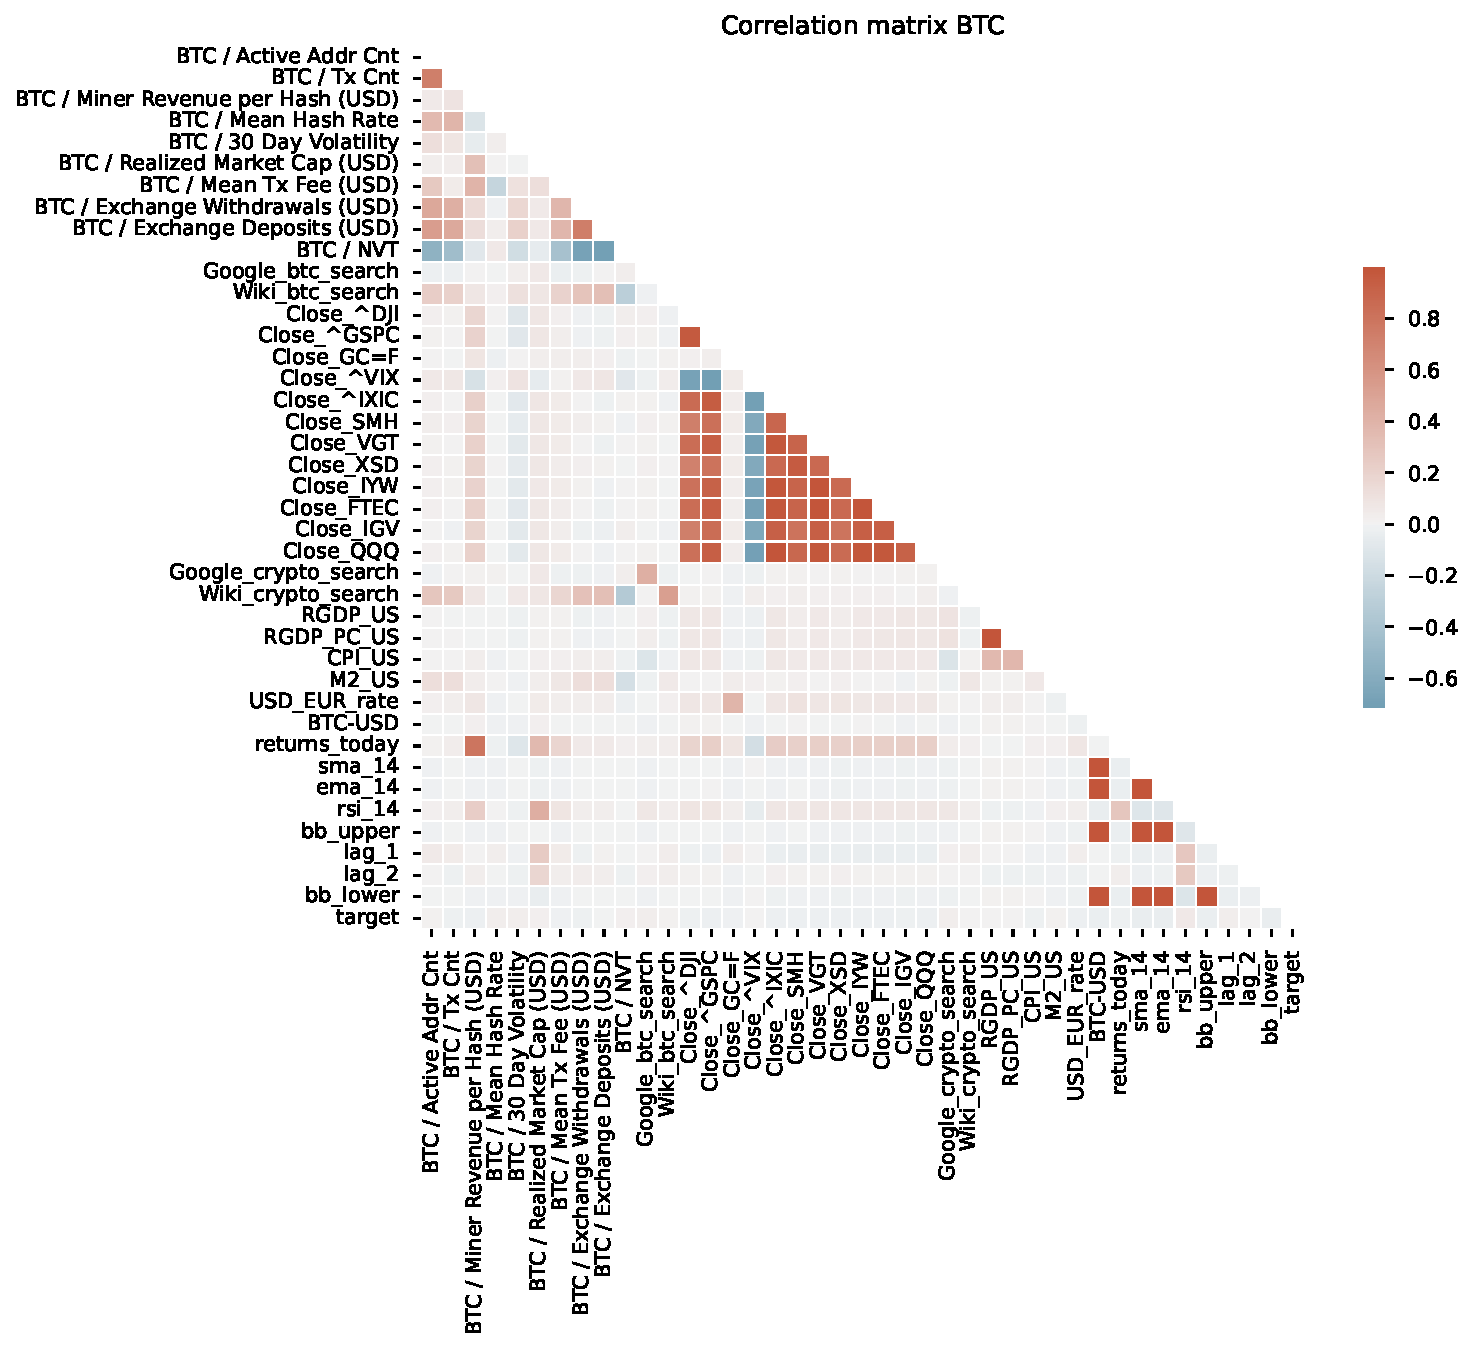
\includegraphics[width=1\textwidth]{Figures/Corr_btc_logdiff.pdf}
    \caption*{Source: Author}
    \label{fig:Corr_btc_logdiff}
\end{figure}




\begin{figure}[!h]
    \centering
    \caption{Learned coefficients of the Ridge regression model
    with incremental training on the BTC dataset. Five 
    coefficients with highest variance are highlighted.}
    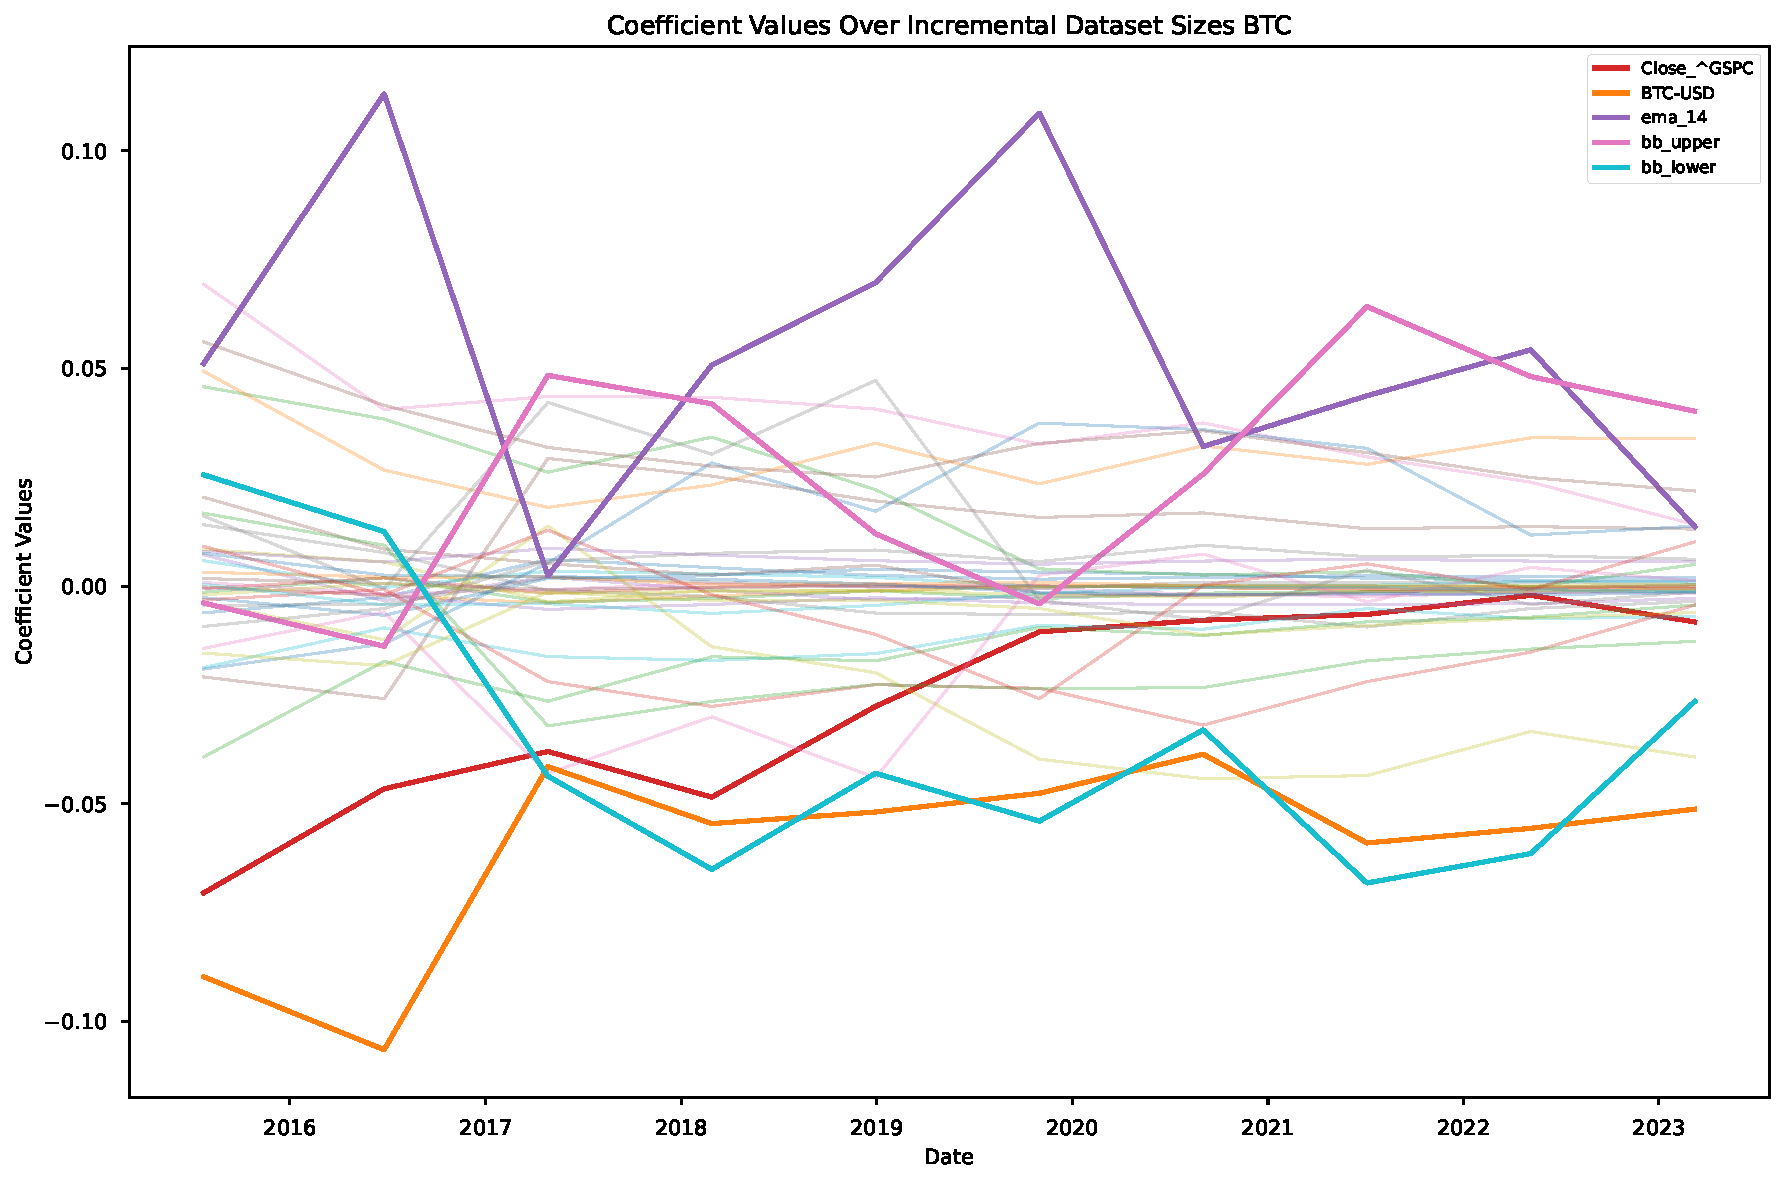
\includegraphics[width=1\textwidth]{Figures/coefficient_values_incremental_btc.pdf}
    \caption*{Source: Author}
    \label{fig:coefs_incremental_btc}
\end{figure}

\begin{figure}[!h]
    \centering
    \caption{Learned coefficients of the Ridge regression model
    with sliding window training on the BTC dataset. Five 
    coefficients with highest variance are highlighted.}
    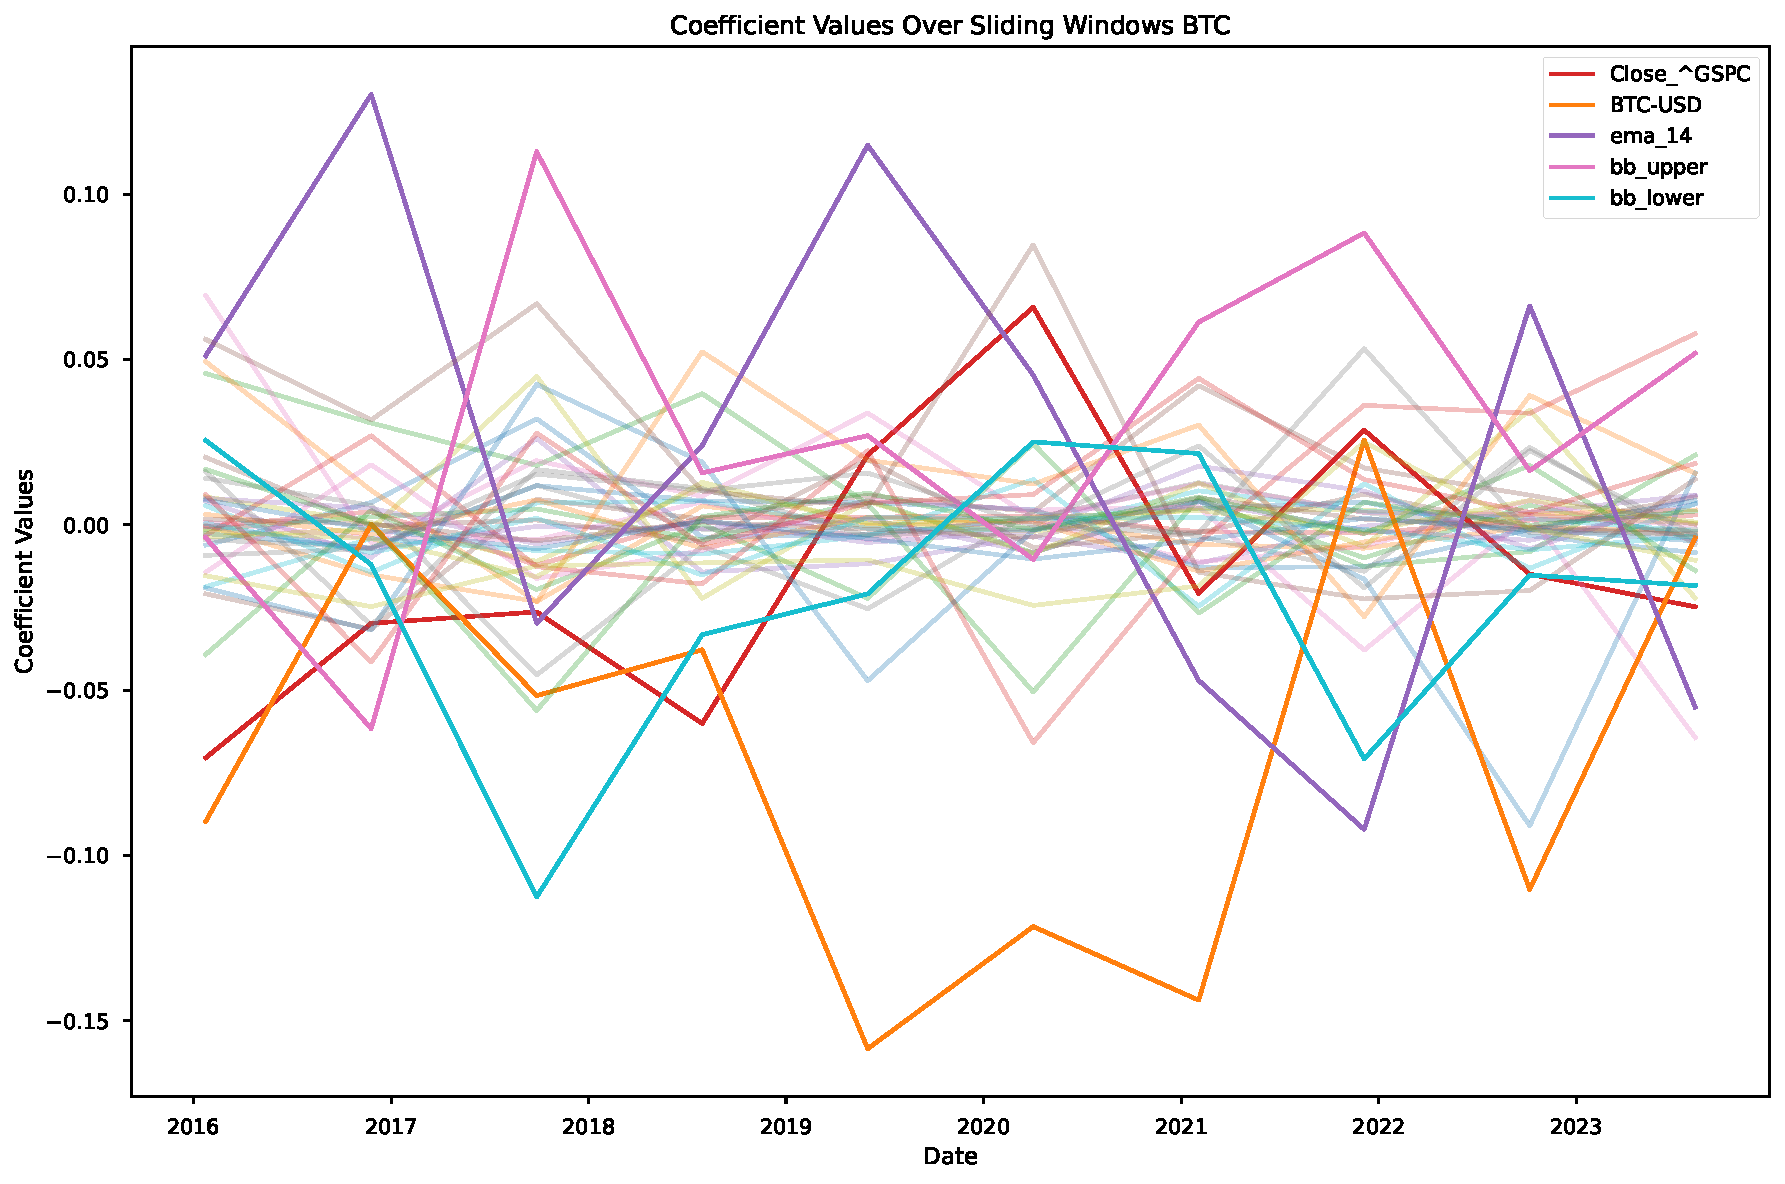
\includegraphics[width=1\textwidth]{Figures/coefficient_values_sliding_btc.pdf}
    \caption*{Source: Author}
    \label{fig:coefs_sliding_btc}
\end{figure}

\section{Limitations}
\label{sec:limitations}

\chapter{Useful Hints}
\label{chap:six}

If you write in English, you might find the following hint
useful: The indefinite article a is used as an before a
vowel sound---for example an apple, an hour, an unusual
thing, an \ac{MNC} (because the acronym is pronounced Em-En-See). Before a consonant sound represented
by a vowel letter a is usual---for example a one, a
unique thing, a historic chance. Few more tips to follow:


\begin{itemize}
\item Don't give orders---don't write in the imperative mood---unless you are training to be a teacher.
\item Avoid the use of questions. You may know the answer: does your reader? It's much safer to tell her, or him.
\item Do not become entangled in the problems of `sexist' language. It is much easier to write in the plural. ``Students should check their work'' is good English. ``A student should check---'' is also good English, but now the problems begin: ``---her work?'' ``---his work?'' Which? You can write ``his or her,'' but that seems clumsy. Stick to the plural.
\item If you must refer to yourself, use the third person such as ``The present writer would recommend that \ldots'' may be useful.
\item Use the full forms of words and phrases, not contractions like ``he's,'' ``don't,'' etc. Keep the apostrophe to indicate possession---and use it correctly. Academics really sneer at students who use the ``Greengrocer's apostrophe.''
\end{itemize}


\begin{itemize}
\item Do not despise short, workmanlike, and effective plain English words. If they mean what you want to say. Accurately.
\item Avoid the use of humor in academic writing---unless you are very sure of yourself.
\item Even when you are not being funny, avoid the use of irony or sarcasm.
\item Paragraphs in academic English should contain more than one sentence. (Short paragraphs look as if you are writing for a tabloid newspaper---or a simple Template!) I guess that the average academic book runs to two or three paragraphs per page. Look at the books in your subject, and get a feel for how long your own paragraphs should be when you are imitating the academic style.
\item Use the word that more in formal writing than most of us do in speech---particularly after such verbs of utterance as to say, to report, to think etc. It can help to make your writing much clearer.
\item Develop an academic vocabulary. The `long words' you learn in the course of your studies are long usually because they have more precise meanings than their less formal equivalents. They are therefore better when you want to be accurate. (Also they allow you to sound like someone who deserves a degree.)
\end{itemize}



\begin{itemize}
\item  Use as few words as you can; but use enough words to express your meaning as fully as you can. Your judgment of what is appropriate here is part of what you should learn throughout your course.
\item  Avoid lazy words such as ``nice''. It is usually better to say ``acquire'' or ``obtain'' than ``get;'' and it may be better, if you mean ``through the use of money,'' to say ``purchase'' or---better still---''buy.''
\item A short word like ``buy'' is better than a long one like ``purchase''---unless the long one is more accurate. A ``statutory instrument'' is better than a ``rule''---to a lawyer, at any rate.
\item Proof-read with care. Ask someone else to help---you may be too close to your work to be able to see your mistakes.
\item If in doubt, choose the more formal, or possibly just the more old-fashioned, of two words. For example, say quotation rather than quote whenever you mean the use of somebody else's words.
\end{itemize}



\begin{itemize}
\item You will often sound more academic if you include doubts in your work---and qualifications. Within the scope of this thesis, the current writer cannot hope to cover all the possible implications of the question.ԍ
\item In this context, the use of litotes sounds very academic. This is the construction where a writer uses a negative with a negative adjective, e.g.\ it is not unlikely that \ldots This does not mean the same as it is probable that \ldots It has a shade of meaning and qualification that can be useful to academic writers.
\end{itemize}





%\chapter{Conclusion}
\label{conclusion}

The conclusion should briefly summarize the problem statement and the general content of the work and the emphasize on the main contribution of the work.

When writing the conclusion keep in mind that some readers may not have gone through the whole thesis, but have jumped directly to the conclusion after having read the abstract in order the decide on the personal relevance of the thesis. Therefore, the conclusion should be self contained, which means that a reader should be able to understand the essence of the conclusion without having to read the whole thesis.

The conclusion typically ends with an outlook that describes possible extensions of the presented approaches and of planned future work.

\clearpage
%-----<<< -------- >>>-----

%-----<<< REFERENCES >>>-----
\fancyhead[LO]{\sffamily Bibliography}					%headers in sans serif and not in uppercase
\bibliographystyle{Styles/Stylebib}							%style of literature, you can use e.g. newapa	instead of Styles/Stylebib
\bibliography{Styles/Bibliography}							%bibliography database
\addcontentsline{toc}{chapter}{Bibliography} 		%Add bibliography to the table of contents
\clearpage
%-----<<< ---------- >>>-----

%-----<<< APPENDIXES >>>-----
\backmatter																			%uppercase roman pagination for back matter; appendices start
\autohdr																				%automatic headers     				
\chapter{Detailed Results Tables}
\label{app:A}
\begin{table}[htbp]
\centering
\caption{Results of the Ridge Regression Model Train Dataset, $R^2$ metric, BTC}
\begin{tabular}{lrrr}
    \toprule
    {} &  BTC-LR - 1 day &  BTC-LR - 5 days &  BTC-LR - 10 days \\
    \midrule
    Full dimensionality   &         0.01330 &          0.03727 &           0.05569 \\
    95\% retained variance &         0.01097 &          0.03391 &           0.03929 \\
    98\% retained variance &         0.01143 &          0.03533 &           0.05464 \\
    99\% retained variance &         0.01189 &          0.03600 &           0.05466 \\
    \bottomrule
\end{tabular}
\end{table}


\begin{table}[htbp]
    \centering
    \caption{Results of the SVR Model Train Dataset, $R^2$ metric, BTC}
\begin{tabular}{lrrr}
    \toprule
    {} &  BTC-SVR - 1 day &  BTC-SVR - 5 days &  BTC-SVR - 10 days \\
    \midrule
    Full dimensionality   &      -0.00226 &          -0.01158 &           -0.01658 \\
    95\% retained variance &      -0.00226 &          -0.01136 &           -0.02180 \\
    98\% retained variance &      -0.00226 &          -0.01154 &           -0.01780 \\
    99\% retained variance &      -0.00226 &          -0.01153 &           -0.01837 \\
    \bottomrule
\end{tabular}
\end{table}

\begin{table}[htbp]
    \centering
    \caption{Results of the LSTM Model Train Dataset, $R^2$ metric, BTC}
\begin{tabular}{lrrr}
    \toprule
    {} &  BTC-LSTM - 1 day &  BTC-LSTM - 5 days &  BTC-LSTM - 10 days \\
    \midrule
    Full dimensionality   &       &           &           \\
    95\% retained variance &       &           &            \\
    98\% retained variance &       &          &            \\
    99\% retained variance &      &       &           \\
    \bottomrule
\end{tabular}
\end{table}

\begin{table}[htbp]
    \centering
    \caption{Results of the Ridge Model Test Dataset, $R^2$ metric, BTC}
\begin{tabular}{lrrr}
    \toprule
    {} &  BTC-LR - 1 day &  BTC-LR - 5 days &  BTC-LR - 10 days\\
    \midrule
    Full dimensionality   &        -0.00484 &         -0.01428 &          -0.04277 \\
    95\% retained variance &         0.00050 &         -0.01568 &          -0.01613\\
    98\% retained variance &        -0.00022 &         -0.01340 &          -0.04184\\
    99\% retained variance &        -0.00170 &         -0.01352 &          -0.04186\\
    \bottomrule
    \end{tabular}
\end{table}

\begin{table}[htbp]
    \centering
    \caption{Results of the SVR Model Test Dataset, $R^2$ metric, BTC}
\begin{tabular}{lrrr}
    \toprule
    {} &  BTC-SVR - 1 day &  BTC-SVR - 5 days &  BTC-SVR - 10 days\\
    \midrule
    Full dimensionality     &  -0.00037 &          -0.00221 &           -0.00667 \\
    95\% retained variance   &  -0.00037 &          -0.00202 &           -0.00368\\
    98\% retained variance   &  -0.00037 &          -0.00243 &           -0.00535\\
    99\% retained variance   &  -0.00037 &          -0.00199 &           -0.00517\\
    \bottomrule
\end{tabular}
\end{table}

\begin{table}[htbp]
    \centering
    \caption{Results of the LSTM Model Test Dataset, $R^2$ metric, BTC}
\begin{tabular}{lrrr}
    \toprule
    {} &  BTC-LSTM - 1 day &  BTC-LSTM - 5 days &  BTC-LSTM - 10 days \\
    \midrule
    Full dimensionality   &       &           &           \\
    95\% retained variance &       &           &            \\
    98\% retained variance &       &          &            \\
    99\% retained variance &      &       &           \\
    \bottomrule
\end{tabular}
\end{table}

%%ETH


\begin{table}[htbp]
    \centering
    \caption{Results of the Ridge Regression Model Train Dataset, $R^2$ metric, ETH}
    \begin{tabular}{lrrr}
        \toprule
        {} &  ETH-LR - 1 day &  ETH-LR - 5 days &  ETH-LR - 10 days \\
        \midrule
        Full dimensionality   &      0.01709    &     0.03234     &        0.04851    \\
        95\% retained variance &     0.01332    &   0.02988 &     0.04177     \\
        98\% retained variance &    0.01373   &     0.0302   &    0.04185  \\
        99\% retained variance &   0.01687    &     0.03137    &  0.04682   \\
        \bottomrule
    \end{tabular}
    \end{table}
    
    
    \begin{table}[htbp]
        \centering
        \caption{Results of the SVR Model Train Dataset, $R^2$ metric, ETH}
    \begin{tabular}{lrrr}
        \toprule
        {} &  ETH-SVR - 1 day &  ETH-SVR - 5 days &  ETH-SVR - 10 days \\
        \midrule
        Full dimensionality   &  -0.00398   &    -0.01759     &   -0.02885       \\
        95\% retained variance &  -0.00398  &    -0.01778     &   -0.02787        \\
        98\% retained variance &  -0.00398   &   -0.0177      &   -0.02888      \\
        99\% retained variance &  -0.00398  &    -0.01748     &  -0.02891   \\
        \bottomrule
    \end{tabular}
    \end{table}
    
    \begin{table}[htbp]
        \centering
        \caption{Results of the LSTM Model Train Dataset, $R^2$ metric, ETH}
    \begin{tabular}{lrrr}
        \toprule
        {} &  ETH-LSTM - 1 day &  ETH-LSTM - 5 days &  ETH-LSTM - 10 days \\
        \midrule
        Full dimensionality   &       &           &           \\
        95\% retained variance &       &           &            \\
        98\% retained variance &       &          &            \\
        99\% retained variance &      &       &           \\
        \bottomrule
    \end{tabular}
    \end{table}
    
    \begin{table}[htbp]
        \centering
        \caption{Results of the Ridge Model Test Dataset, $R^2$ metric, ETH}
    \begin{tabular}{lrrr}
        \toprule
        {} &  ETH-LR - 1 day &  ETH-LR - 5 days &  ETH-LR - 10 days\\
        \midrule
        Full dimensionality   &   -0.0029   &    -0.02056   &    -0.02534    \\
        95\% retained variance &   -0.00278  &    -0.01793    &     -0.0089   \\
        98\% retained variance &    -0.00212    &     -0.01892    &    -0.00918  \\
        99\% retained variance &     -0.00267  &    -0.02003   &    -0.02768   \\
        \bottomrule
        \end{tabular}
    \end{table}
    
    \begin{table}[htbp]
        \centering
        \caption{Results of the SVR Model Test Dataset, $R^2$ metric, ETH}
    \begin{tabular}{lrrr}
        \toprule
        {} &  ETH-SVR - 1 day &  ETH-SVR - 5 days &  ETH-SVR - 10 days\\
        \midrule
        Full dimensionality     & -0.0022 &    -0.00038    &    0.00065     \\
        95\% retained variance   & -0.00219 &    -0.0006   &     0.00065   \\
        98\% retained variance   & -0.0022  &      -0.00047   &     0.00058     \\
        99\% retained variance   &  -0.0022 &      -0.00011   &    0.00059    \\
        \bottomrule
    \end{tabular}
    \end{table}
    
    \begin{table}[htbp]
        \centering
        \caption{Results of the LSTM Model Test Dataset, $R^2$ metric, ETH}
    \begin{tabular}{lrrr}
        \toprule
        {} &  ETH-LSTM - 1 day &  ETH-LSTM - 5 days &  ETH-LSTM - 10 days \\
        \midrule
        Full dimensionality   &       &           &           \\
        95\% retained variance &       &           &            \\
        98\% retained variance &       &          &            \\
        99\% retained variance &      &       &           \\
        \bottomrule
    \end{tabular}
    \end{table}
    

%%LTC

\begin{table}[htbp]
    \centering
    \caption{Results of the Ridge Regression Model Train Dataset, $R^2$ metric, LTC}
    \begin{tabular}{lrrr}
        \toprule
        {} &  LTC-LR - 1 day &  LTC-LR - 5 days &  LTC-LR - 10 days \\
        \midrule
        Full dimensionality   &    0.00985      &   0.03449       &     0.05824       \\
        95\% retained variance &    0.00921     & 0.03073   &       0.03773    \\
        98\% retained variance &     0.0093  &       0.03362 &    0.0463  \\
        99\% retained variance &    0.00956   &     0.03425    &   0.04657  \\
        \bottomrule
    \end{tabular}
    \end{table}
    
    
    \begin{table}[htbp]
        \centering
        \caption{Results of the SVR Model Train Dataset, $R^2$ metric, LTC}
    \begin{tabular}{lrrr}
        \toprule
        {} &  LTC-SVR - 1 day &  LTC-SVR - 5 days &  LTC-SVR - 10 days \\
        \midrule
        Full dimensionality   &   -0.00056  &    0.00795     &    -0.00501     \\
        95\% retained variance &   -0.00056 &     -0.00291    &      -0.00502     \\
        98\% retained variance &  -0.00056   &     -0.00283    &     0.00095    \\
        99\% retained variance &  -0.00056  &    -0.00291     &   -0.00501  \\
        \bottomrule
    \end{tabular}
    \end{table}
    
    \begin{table}[htbp]
        \centering
        \caption{Results of the LSTM Model Train Dataset, $R^2$ metric, LTC}
    \begin{tabular}{lrrr}
        \toprule
        {} &  LTC-LSTM - 1 day &  LTC-LSTM - 5 days &  LTC-LSTM - 10 days \\
        \midrule
        Full dimensionality   &       &           &           \\
        95\% retained variance &       &           &            \\
        98\% retained variance &       &          &            \\
        99\% retained variance &      &       &           \\
        \bottomrule
    \end{tabular}
    \end{table}
    
    \begin{table}[htbp]
        \centering
        \caption{Results of the Ridge Model Test Dataset, $R^2$ metric, LTC}
    \begin{tabular}{lrrr}
        \toprule
        {} &  LTC-LR - 1 day &  LTC-LR - 5 days &  LTC-LR - 10 days\\
        \midrule
        Full dimensionality   &    0.00293  &   -0.00597    &     -0.06626    \\
        95\% retained variance &   0.00398  &   -0.00194     &      -0.0241  \\
        98\% retained variance &    0.00347    &   -0.00486      &  -0.01171    \\
        99\% retained variance &   0.00297    &    -0.00495   &    -0.00956   \\
        \bottomrule
        \end{tabular}
    \end{table}
    
    \begin{table}[htbp]
        \centering
        \caption{Results of the SVR Model Test Dataset, $R^2$ metric, LTC}
    \begin{tabular}{lrrr}
        \toprule
        {} &  LTC-SVR - 1 day &  LTC-SVR - 5 days &  LTC-SVR - 10 days\\
        \midrule
        Full dimensionality     & -0.00035 &    0.00435    &    -0.00409     \\
        95\% retained variance   & -0.00035 &   -0.00195    &      -0.0041  \\
        98\% retained variance   & -0.00035  &      -0.00198   &    -0.00213      \\
        99\% retained variance   &  -0.00035 &    -0.00194     &    -0.00409    \\
        \bottomrule
    \end{tabular}
    \end{table}
    
    \begin{table}[htbp]
        \centering
        \caption{Results of the LSTM Model Test Dataset, $R^2$ metric, LTC}
    \begin{tabular}{lrrr}
        \toprule
        {} &  LTC-LSTM - 1 day &  LTC-LSTM - 5 days &  LTC-LSTM - 10 days \\
        \midrule
        Full dimensionality   &       &           &           \\
        95\% retained variance &       &           &            \\
        98\% retained variance &       &          &            \\
        99\% retained variance &      &       &           \\
        \bottomrule
    \end{tabular}
    \end{table}
               			%input file

\chapter{Additional Figures}

\begin{document}[!htbp]
    \begin{center}
    \caption{Missing Values BTC before subseting}
    \label{fig:btc_missing_1}
    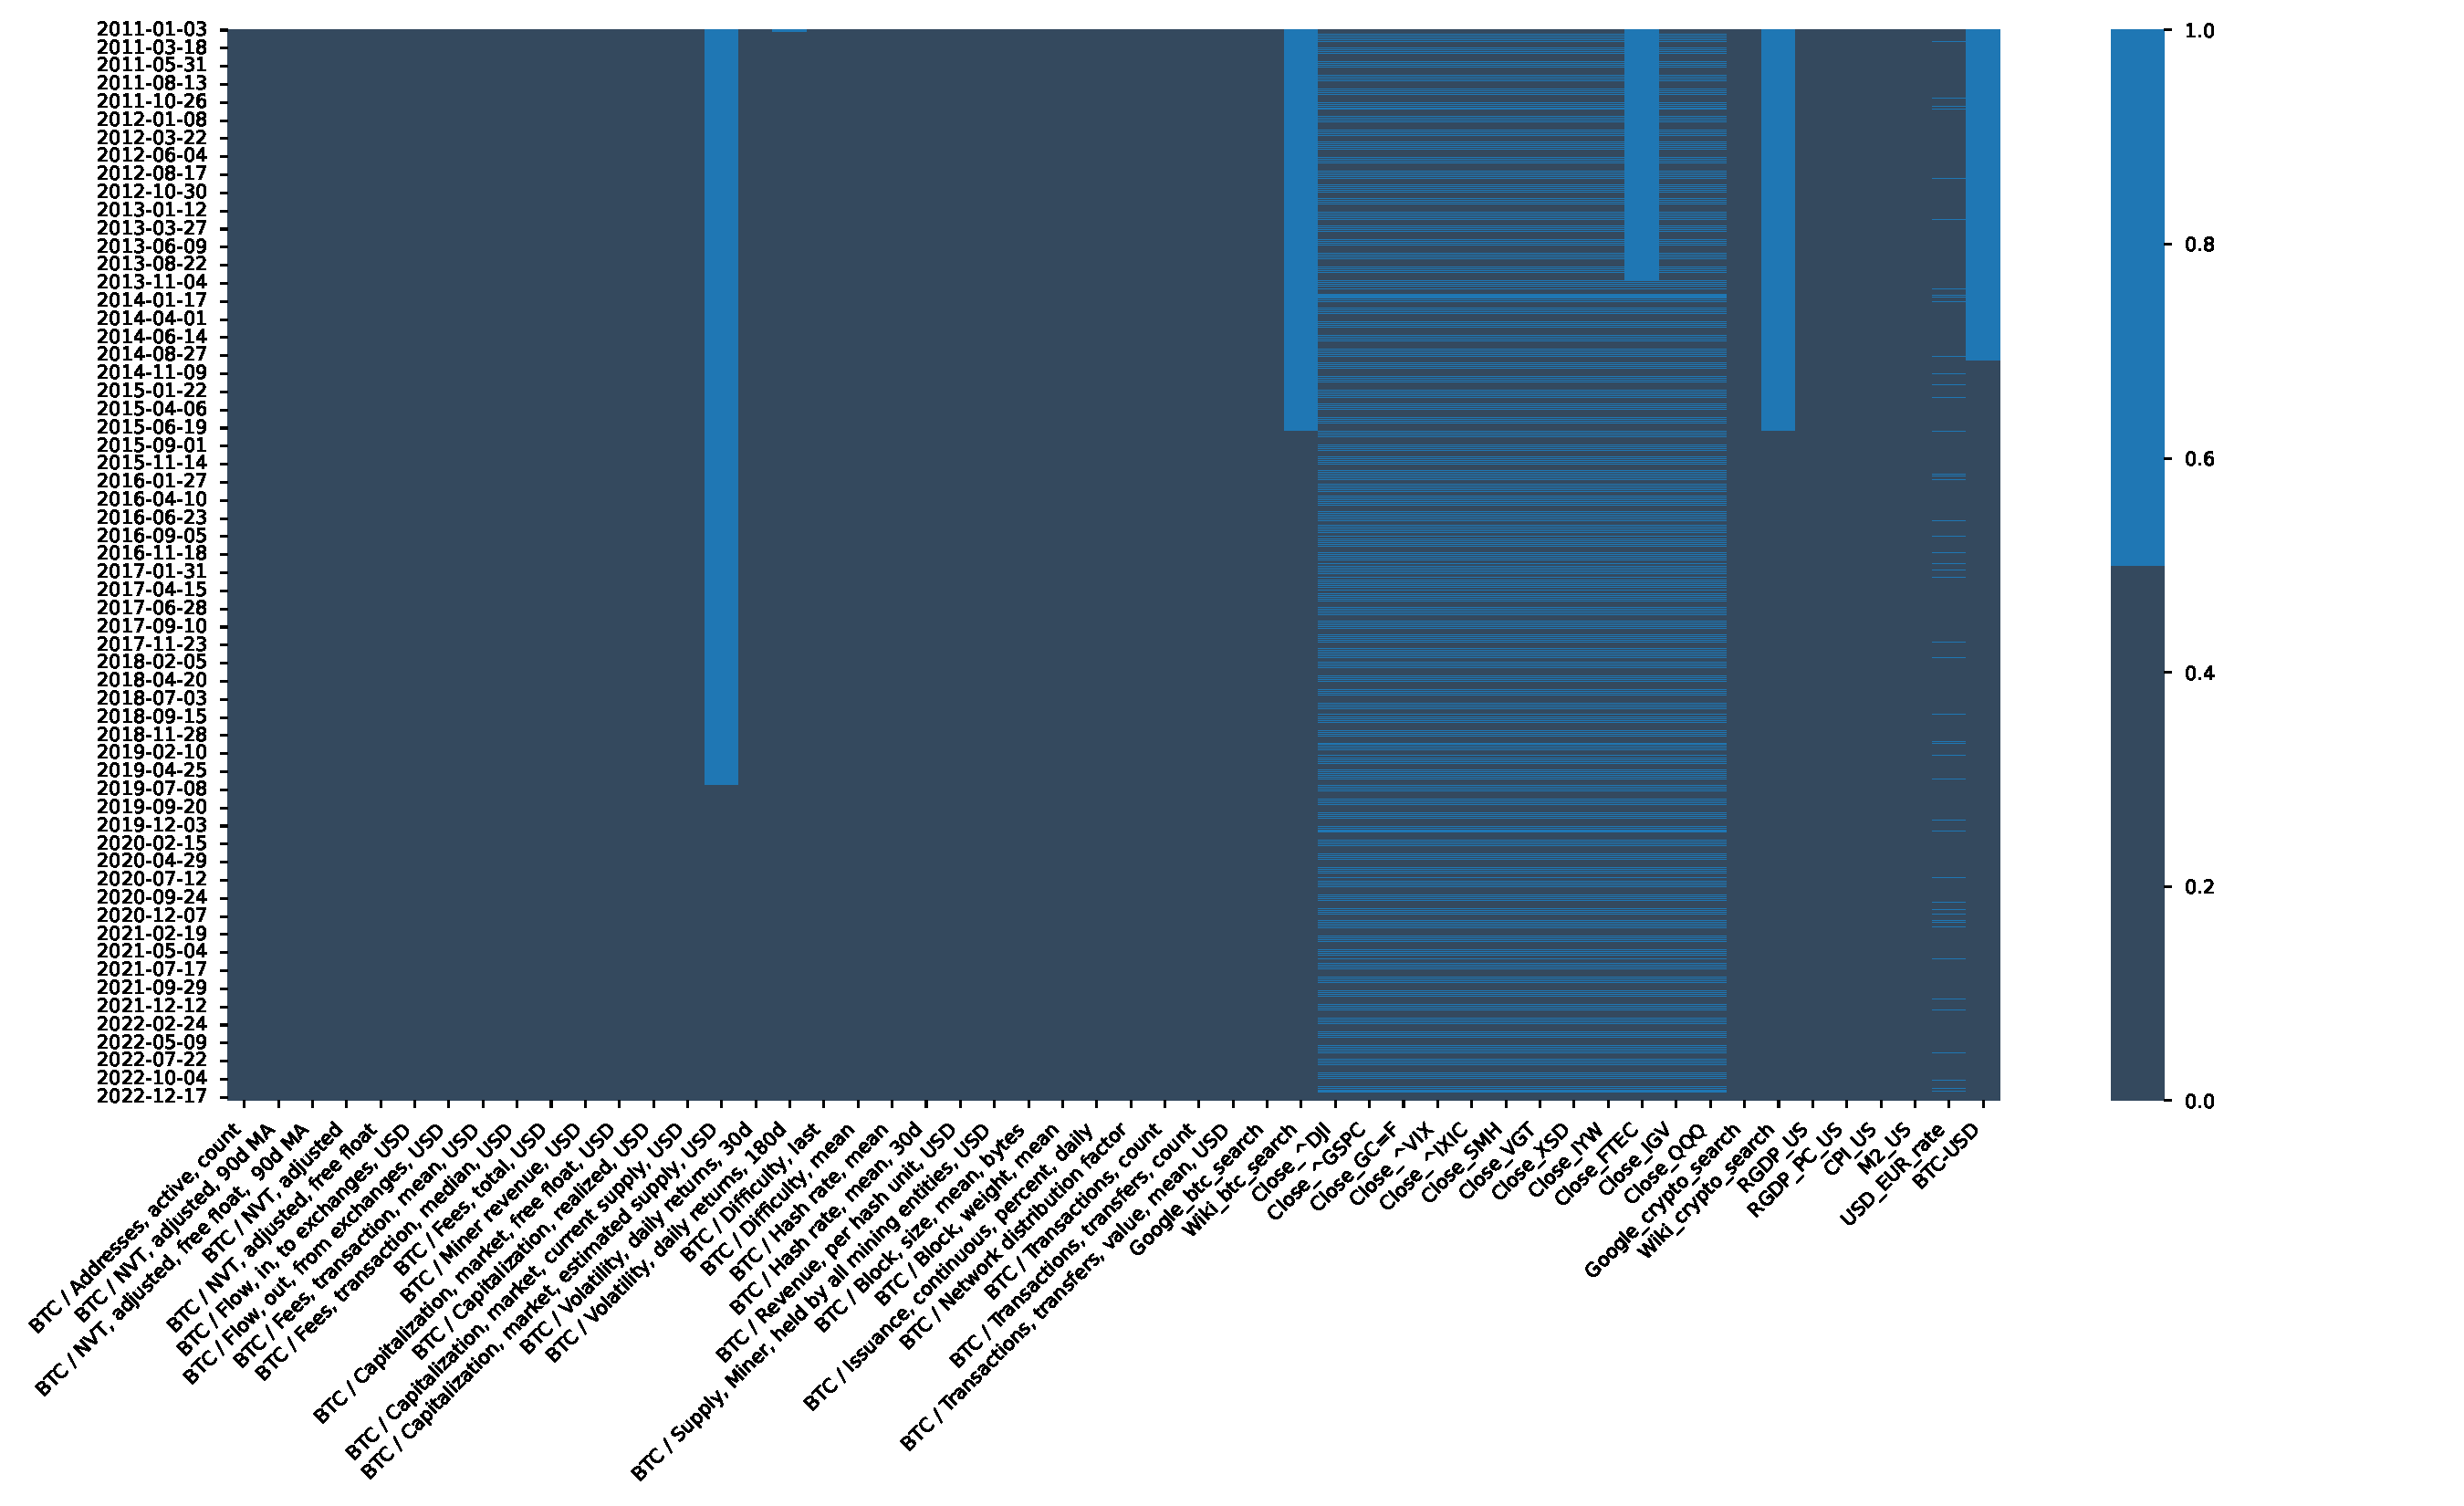
\includegraphics[max size={\textwidth}{\textheight}]{Figures/BTC_missing_1.pdf}
    \end{center}\vspace{-0.5cm}
    \begin{source}Author\end{source}
    \end{document}           			%input file

\chapter{Variables Description}
\label{app:var_desc}
Following is the list of technical variables on the example of \ac{BTC}. The definitions were taken
directly from \textbf{\href{https://charts.coinmetrics.io/crypto-data/}{coinmetrics.io}} to avoid any misconceptions:

\begin{itemize}
    \item \textit{BTC / Addresses, active, count} - The sum count of unique addresses that were active in the network (either as a recipient or originator of a ledger change) that interval. All parties in a ledger change action (recipients and originators) are counted. Individual addresses are not double-counted if previously active.
    \item \textit{BTC / NVT, adjusted, 90d MA} - The ratio of the network value (or market capitalization, current supply) to the 90-day moving average of the adjusted transfer value. Also referred to as NVT.
    \item \textit{BTC / NVT, adjusted, free float,  90d MA} - The ratio of the free float network value (or market capitalization, free float) to the 90-day moving average of the adjusted transfer value.
    \item \textit{BTC / NVT, adjusted} - The ratio of the network value (or market capitalization, current supply) divided by the adjusted transfer value. Also referred to as NVT.
    \item \textit{BTC / NVT, adjusted, free float} - The ratio of the free float network value (or market capitalization, free float) divided by the adjusted transfer value. Also referred to as FFNVT.
    \item \textit{BTC / Flow, in, to exchanges, USD} - The sum USD value sent to exchanges that interval, excluding exchange to exchange activity.
    \item \textit{BTC / Flow, out, from exchanges, USD} - The sum USD value withdrawn from exchanges that interval, excluding exchange to exchange activity.
    \item \textit{BTC / Fees, transaction, mean, USD} - The USD value of the mean fee per transaction that interval.
    \item \textit{BTC / Fees, transaction, median, USD} - The USD value of the median fee per transaction that interval.
    \item \textit{BTC / Fees, total, USD} - The sum USD value of all fees paid by transactors that interval. Fees do not include new issuance.
    \item \textit{BTC / Miner revenue, USD} - The USD value of the mean miner reward per estimated hash unit performed during the period, also known as hashprice. The unit of hashpower measurement depends on the protocol.
    \item \textit{BTC / Capitalization, market, free float, USD} - The ratio of the free float market capitalization to the sum realized USD value of the current supply.
    \item \textit{BTC / Capitalization, realized, USD} - The sum USD value based on the USD closing price on the day that a native unit last moved (i.e., last transacted) for all native units.
    \item \textit{BTC / Capitalization, market, current supply, USD} - The sum USD value of the current supply. Also referred to as network value or market capitalization.
    \item \textit{BTC / Capitalization, market, estimated supply, USD} - The sum USD value of the estimated supply in circulation. Also referred to as network value or market capitalization.
    \item \textit{BTC / Volatility, daily returns, 30d} - The 30D volatility, measured as the standard deviation of the natural log of daily returns over the past 30 days.
    \item \textit{BTC / Volatility, daily returns, 180d} - The 180D volatility, measured as the standard deviation of the natural log of daily returns over the past 180 days.
    \item \textit{BTC / Difficulty, last} - The difficulty of the last block in the interval. Difficulty represents how hard it is to find a hash that meets the protocol-designated requirement (i.e., the difficulty of finding a new block) that day. The requirement is unique to each applicable cryptocurrency protocol. Difficulty is adjusted periodically by the protocol as a function of how much hashing power is being deployed by miners.
    \item \textit{BTC / Difficulty, mean} - The mean difficulty of finding a hash that meets the protocol-designated requirement (i.e., the difficulty of finding a new block) that interval. The requirement is unique to each applicable cryptocurrency protocol. Difficulty is adjusted periodically by the protocol as a function of how much hashing power is being deployed by miners.
    \item \textit{BTC / Hash rate, mean} - The mean rate at which miners are solving hashes that interval. Hash rate is the speed at which computations are being completed across all miners in the network. The unit of measurement varies depending on the protocol.
    \item \textit{BTC / Hash rate, mean, 30d} - The mean rate at which miners are solving hashes over the last 30 days. Hash rate is the speed at which computations are being completed across all miners in the network. The unit of measurement varies depending on the protocol
    \item \textit{BTC / Revenue, per hash unit, USD} - The USD value of the mean miner reward per estimated hash unit performed during the period, also known as hashprice. The unit of hashpower measurement depends on the protocol.
    \item \textit{BTC / Supply, Miner, held by all mining entities, USD} - The sum of the balances of all mining entities in USD. A mining entity is defined as an address that has been credited from a transaction debiting the 'FEES' or 'ISSUANCE' accounts.
    \item \textit{BTC / Block, size, mean, bytes} - The mean size (in bytes) of all blocks created that day.
    \item \textit{BTC / Block, weight, mean} - The mean weight of all blocks created that day. Weight is a dimensionless measure of a block’s “size”. It is only applicable for chains that use SegWit (segregated witness).
    \item \textit{BTC / Issuance, continuous, percent, daily} - The percentage of new native units (continuous) issued over that interval divided by the current supply at the end of that interval. Also referred to as the daily inflation rate.
    \item \textit{BTC / Network distribution factor} - The ratio of supply held by addresses with at least one ten-thousandth of the current supply of native units to the current supply.
    \item \textit{BTC / Transactions, count} - The sum count of transactions that interval. Transactions represent a bundle of intended actions to alter the ledger initiated by a user (human or machine). Transactions are counted whether they execute or not and whether they result in the transfer of native units or not (a transaction can result in no, one, or many transfers). Changes to the ledger mandated by the protocol (and not by a user) or post-launch new issuance issued by a founder or controlling entity are not included here.
    \item \textit{BTC / Transactions, transfers, count} - The sum count of transfers that interval. Transfers represent movements of native units from one ledger entity to another distinct ledger entity. Only transfers that are the result of a transaction and that have a positive (non-zero) value are counted.
    \item \textit{BTC / Transactions, transfers, value, mean, USD} - The sum USD value of native units transferred divided by the count of transfers (i.e., the mean size in USD of a transfer) between distinct addresses that interval.
\end{itemize}

\chapter{Aditional Contents}

All of the source codes and data to reproduce the results are 
available at: \href{https://github.com/Tomas-Barhon/Noise-reduction-and-feature-extraction-with-principal-component-analysis}{Noise-reduction-and-feature-extraction}. 
Including all the instructions on how to install the necessary dependencies.


\clearpage
%-----<<< --------- >>>-----


\end{document}
%-----<<<<<<<<< END OF DOCUMENT >>>>>>>>>-----
